\documentclass[11pt,a4paper]{article}
%\usepackage[utf8]{inputenc}
%\usepackage[ascii]{inputenc}
\usepackage{geometry}
\usepackage[dvipsnames]{xcolor}
\usepackage{textcomp}
\usepackage{graphicx}
\usepackage{caption}
\usepackage{subcaption}
\usepackage{amsmath}
\usepackage{tikz}

\begin{document}

\tableofcontents

\section*{Introduction}
Objectif du cours : 
\begin{itemize}
\item Rappel des notions de bases de traitement du signal 
\item Design et synthèse de filtre 
\item Applications sous MATLAB/GNU Octave
\end{itemize}

Ce cours sera principalement formulé sous forme de réponse à des questions précises généralement couplées à des questions techniques sur le sujet.

\section{Fondamentaux}
\subsection{Traitement du signal}
Le traitement du signal est le champ de l'ingénierie qui concerne les outils physiques et mathématiques mis en œuvre pour la transmission de l'information suivant des contraintes précises.\\

On peut définir le signal de la façon suivante: "Le signal est le support de l’information émise par une source et destinée à un récepteur." (M. Bellanger, \textit{Traitement numérique du signal, 2012}). La problématique de base étant que, bien souvent, l'information peut voir son contenu dégradé par divers mécanismes entre la source et le récepteur. Le traitement du signal, qu'il soit analogique ou numérique, va alors souvent consister à extraire ou conserver l'information entre ces deux points d'intérêt.\\

L'information peut ici prendre plusieurs formes physiques différentes. Il peut s'agir d'une onde électromagnétique se propageant dans le vide, l'air ou encore un cable. Il peut également s'agir d'un champ de pression ou de déformation. L'information peut également être "codée" comme c'est le cas des signaux numériques par opposition aux signaux analogiques.\\

\textbf{Question: Exemple de traitement du signal analogique et numérique dans la vide quotidienne ?}\\

Le traitement du signal est basé sur la connaissance des mécanismes physiques à l’œuvre dans la propagation du signal (acoustique, électromagnétisme, etc...) et sur des outils mathématiques (statistiques, analyse de fonctions) permettant à la fois d'extraire des caractéristiques du signal ou de les modifier de manière contrôlée. Cette opération est souvent réalisée à l'aide de ce qu'on appelle des filtres. \\
 
\subsection{Qu'est ce qu'un filtre ?}
"En traitement du signal, un filtre est un dispositif ou un processus permettant de retirer des composantes ou des parties indésirables d'un signal." (/en.wikipedia.org/wiki/Filter (signal processing))\\

\vspace{0.5cm}

\begin{center}
	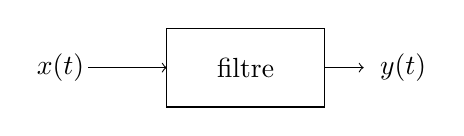
\begin{tikzpicture}
	%\draw (2.15,-1.5) node {Glc};
	%\draw[->] (2.15,-1)-- (2.15,-0.5);
	%\draw (1.25,-0.5) rectangle(3,0.5);
	\draw (2.15,0) node {$x(t)$};
	%\draw[->] (2.15,0.5)-- (2.15,1);
	%\draw (2.15,1.5) node {ATP};
	
	\draw[->] (2.5,0)-- (3.5,0);
	\draw (3.5,-0.5) rectangle(5.5,0.5) ;
	\draw (4.5,0) node {filtre};
	%\draw[->] (4.5,0.5) arc(90:60:0.5);
	%\draw[->] (4.5,-0.5) arc(-90:-120:0.5);
	%\draw[->] (4.5,-1)-- (4.5,-0.5);
	%\draw (4.5,-1.5) node {Glt};
	%\draw[->] (4.5,0.5)-- (4.5,1);
	%\draw (4.5,1.5) node {ATP};
	
	\draw[->] (5.5,0)-- (6,0);
	%\draw[->] (6,-0.5) rectangle(7,0.5); 
	\draw (6.5,0) node {$y(t)$};
	%\draw[->] (6.5,-1)-- (6.5,-0.5);
	%\draw (6.5,-1.5) node {O$_2$};
	%\draw[->] (6.5,0.5)-- (6.5,1);
	%\draw (6.5,1.5) node {ATP};
	\end{tikzpicture}
\end{center}

\vspace{0.5cm}

On note que, dans le cadre plus large de l'ingénierie des systèmes, ce formalisme entrée-sortie est régulièrement employé comme par exemple en automatique, où le but est cette fois d'arriver à obtenir une variable de sortie précise en agissant sur la variable d'entrée. D'ailleurs, les éléments de bases du formalisme mathématique sont les mêmes. Qu'il s'agisse d'un "filtre" ou d'un "système" la base théorique a pour objectif de prédire la réponse du système. Cette notion de prédiction/traitement/commande amène naturellement à la grande question suivante.

\subsection{Comment caractériser un filtre ou un système ?}  
\textbf{Question: Quelles notions/mots clés sont associées pour vous à la caractérisation d'un filtre ou d'un système ?}\\

De nombreuses notions plus ou moins intuitives peuvent être employées pour décrire l'action, souhaitée ou effective, d'un filtre/système, et ces dernières sont souvent au cœur de la conception du filtre/système en question.\\

La notion la plus évidente, déjà abordée par le passé, est la question analogique/numérique. Et cette première subdivision en conditionne d'autres. Dans le cas des signaux analogiques, on distingue régulièrement les filtres "actifs" des filtres "passifs". Un filtre actif est un filtre qui utilise une source d'énergie externe pour amplifier tout ou partie du signal. L'objectif est souvent d'obtenir un meilleur rapport signal-sur-bruit. Dans le cas des filtres numériques, on peut prendre comme premier exemple la notion de causalité. Un filtre numérique non-causal est un filtre qui va utiliser des échantillons du "futur" dans son algorithme de traitement. Un tel filtre ne peut évidemment effectuer un traitement en temps réel et n'est réalisable qu'à l'aide d'une mémoire embarquée associée.\\

Mais avant ces deux notions plutôt intuitives, il y a deux caractéristiques importantes des filtres qui sous-tendent une grande partie des outils mathématiques présentés dans ce cours. Au vu de leur importance globale et de leur aspect moins intuitif (car plus mathématique et calculatoire) on prendra le temps de présenter et de discuter en détail ces deux notions: la \textbf{linéarité} et l'\textbf{invariance dans le temps}.

\subsection{Notion de linéarité}
\textbf{Question: Que veut dire linéaire en ingénierie des systèmes/automatique/traitement du signal ?}\\

La notion de linéarité est un concept majeur en mathématiques et aussi en physique où l'outil mathématique est régulièrement utilisé. Elle peut s'écrire mathématiquement comme suit: soit $f$ une fonction 1D d'une variable réelle,  et soit $x_1$ et $x_2$ et $a$, trois nombres réels, alors:

\[f(a x_1 + x_2) = a f(x_1) + f(x_2)  \] 

\textbf{Linéarité : application}
\textbf{Soit $x$ une variable réelle, les fonctions suivantes sont-elles linéaires ?}:
\begin{itemize}
\item $f(x) = a x^2 + b x + c$ (avec $a$, $b$ et $c$ des constantes réelles positives) 
\item $f(x) = \sqrt{x^2}$
\item $f(x) = a$
\item $f(x) = \ln(x)$
\item $f(x) = \frac{1}{a x + b}$
\end{itemize}

Maintenant que le concept de linéarité a été introduit et/ou rappelé, on peut discuter de son importance en physique et ingénierie. Dans ces deux domaines on se place soit dans un cas linéaire, soit on traite l'objet d'étude de façon à rendre au moins partiellement applicable l'hypothèse de linéarité. En physique cela implique qu'on utilise régulièrement la notion de développement limité. L'un des usages des développement limités étant de remplacer une fonction non linéaire par une approximation linéaire de cette dernière afin de faciliter les calculs.\\

En résumé, si un système est linéaire, la décomposition de son signal de sortie comme somme d'entrée élémentaire est pertinente. Ce qui va s'avérer important plus tard notamment lorsque la théorie de Fourier entrera en jeu.

\subsection{Notion d'invariance dans le temps}
Afin de discuter la notion d'invariance dans le temps il est utile de rappeler la notion de retard ou décalage temporel d'une fonction sous sa forme mathématique.\\

\textbf{Question: Comment s'exprime la notion de retard en mathématiques ?}\\

Un exemple simple est de prendre la fonction exponentielle: exp$(x)$. On sait que exp$(0) = 1$ et exp$(1) = e$. Si on s'intéresse maintenant à la fonction exp$(x-\tau)$ et qu'on recherche les mêmes points particuliers, on retrouve la valeur 1 pour $x = \tau$ et la valeur $e$ pour $x= \tau + 1$. On se rend compte qu'en remplaçant exp$(x)$ par exp$(x-\tau)$, on décale la fonction de $\tau$ suivant les $x$ croissants.  

De façon plus générale, soit $f$ une fonction d'une variable réelle $x$. alors la fonction $g(x) = f(x-\tau)$ correspond à $f(x)$ avec un retard $\tau$. Cette définition correspond aux fonctions continues mais s'applique de façon analogue aux signaux discrets. L'équivalent discret d'une fonction est généralement appelé "suite". Soit $u(n)$, une suite pouvant représenter un signal, la suite $u(n-m)$, où $m$ est un entier, correspond à la suite $u(n)$ décalée de $m$ échantillons. \\

L'invariance dans le temps d'un filtre/système s'exprime alors de la façon suivante: Soit un filtre/système faisant correspondre une sortie $y(t)$ à une entrée $x(t)$. Soit $\tau$ un réel, le filtre/système est dit invariant dans le temps si quelque soit $\tau$, le système fait correspondre la sortie $y(t-\tau)$ à l'entrée $x(t-\tau)$.\\

On peut reformuler en disant que la réponse d'un filtre/système invariant dans le temps ne doit pas dépendre du moment où on l'utilise.\\

\subsection{Capteur linéaire et invariant dans le temps}
Un autre domaine très lié au traitement du signal et où la linéarité est importante est le domaine des \textbf{capteurs}. Un capteur peut être défini de la façon suivante: "Dispositif permettant de capter un phénomène physique et de le restituer sous forme de signal."(Dictonnaire "Le Robert") ou encore comme "Un capteur est un dispositif transformant l'état d'une grandeur physique observée en une grandeur utilisable, telle qu'une tension électrique, une hauteur de mercure, un courant électrique ou la déviation d'une aiguille."\\

\textbf{Question: Que vous évoque la notion de linéarité d'un capteur ?}\\

La linéarité d'un capteur est équivalente à celle présentée pour celle d'un filtre/système. Si on injecte la somme de deux signaux d'entrée $x_1(t)$ et $x_2(t)$, alors la sortie mesurée doit être la somme des sorties $y_1(t)$ et $y_2(t)$ qu'on mesurerait séparément. Dans les faits, un grand nombre de capteurs ne remplissent cette condition que sur une certaines plages de valeur d'entrée.\\

\textbf{Discussion: Plage de linéarité : exemple du ressort}

\subsection{Système linéaire et invariant dans le temps, et réponse impulsionnelle}
Pour démarrer cette partie, on doit définir la notion d'impulsion de Dirac noté $\delta(t)$. Cette dernière peut être vu que comme le cas limite mathématique d'une impulsion de largeur finie. Sur un plan purement mathématique la distribution de Dirac (et la notion de distribution en général) permet de définir la dérivée de fonction comme l'échelon de Heaviside.  De cette définition mathématique découle une possibilité très signifiante dans le cadre de l'ingénierie des systèmes. Elle permet, pour les systèmes linéaires  et invariants dans le temps, d'écrire la relation suivante:\\  
 
\[y(t) = \int^{\infty}_{-\infty} h(\tau) x(t-\tau) \; d\tau = h(t) \star x(t)\] \\

Où $y(t)$ est le signal de sortie, $x(t)$ celui d'entrée et $h(t)$ la réponse impulsionnelle du système. La réponse impulsionnelle du système est défini comme la sortie d'un système lorsque celui reçoit une impulsion de Dirac en entrée.

\begin{center}
	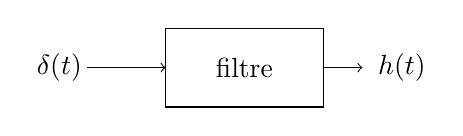
\begin{tikzpicture}

	\draw (2.15,0) node {$\delta(t)$};

	\draw[->] (2.5,0)-- (3.5,0);
	\draw (3.5,-0.5) rectangle(5.5,0.5) ;
	\draw (4.5,0) node {filtre};

	
	\draw[->] (5.5,0)-- (6,0);
	\draw (6.5,0) node {$h(t)$};

	\end{tikzpicture}
\end{center}

Cette équation est appelée \textbf{équation de convolution du filtre}, puisque, comme le montre le membre de droite de l'équation précédente, la sortie du filtre s'écrit comme le produit de convolution du signal d'entrée et de la \textbf{réponse impulsionnelle du filtre}. Les équations précédentes sont valables pour les fonctions continues. Un équivalent existe dans le domaine discret: \\

\[y(n) = \Sigma^{\infty}_{-\infty} h(m) x(n-m) = h(n) \star x(n)\]\\

Les fonctions d'entrée et de sortie et la réponse impulsionnelle, sont alors remplacées par des suites et l'intégrale, somme continue, est remplacée par une somme discrète. Un derniers point est la fonction de Dirac qui dans le domaine discret a pour équivalent \textbf{l'impulsion de Kronecker}\\ 

Les concepts mathématiques introduits dans les paragraphes précédents constituent la base sur laquelle reposent presque intégralement les notions qui vont être présentées dans les sections suivantes de ce cours.

\section{Outils et concepts Mathématiques}

\subsection{Transformée de Laplace} 

\textbf{Question: Que vous évoque la transformée de Laplace ? à quoi sert-elle ?}\\

La transformée de Laplace qui transforme une fonction (ici $f$) d'une \textbf{variable réelle} (ici $t$) en une fonction $L{f}$ d'une \textbf{variable complexe} (ici $p$) et définie par la relation mathématique suivante :

\[L{f}(p) = \int^{\infty}_{0} f(t) e^{-pt} \; dt\] 

Avant d'aller plus loin dans le développement mathématique de cette notion, on va d'abord évoquer son utilité. L'intérêt principal de la transformée de Laplace est de simplifier des opérations mathématiques. Elle permet notamment de remplacer une opération de \textbf{convolution} entre deux fonctions par une multiplication. Elle permet également de simplifier la résolution d'un grand nombre d'équations différentielles ordinaires. On peut être tenté de dire que le problème est simplement déplacé, puisqu'au lieu d'intégrer l'équation différentielle en elle-même on calcule une autre intégrale pour obtenir sa transformée. Cependant il faut comprendre que l'obtention de la transformée est souvent bien plus simple que le calcul direct, et ce car les transformées d'un grand nombre de fonctions sont connues.\\

Pour donner un peu de sens à tout cela, les transformées de Laplace de quelques fonctions usuelles vont être calculées. Ce calcul explicite a plus pour but de manipuler les concepts et les outils mathématiques. Par la suite les transformées seront dans un tableau qu'on pourra consulter quand elle ne seront pas directement calculées par  ordinateur.\\

\textbf{Exercice: Calculer les transformées de Laplace suivantes}\\

\begin{itemize}
\item $\delta (t)$ (impulsion de dirac) 
\item $u(t)$ (échelon de heaviside)
\item $r(t) = t$ (rampe)
\item $f(t) = e^{-at}$ (exponentielle décroissante)
\item $sin(\omega t)$
\end{itemize}

\paragraph{\textbf{1.} $\delta (t)$}
\[L{\delta}(p) = \int^{\infty}_{0} \delta(t) e^{-pt} \; dt = 1\] 
La démonstration de cette dernière est laissée de côté à cause des spécificités de la distribution de Dirac et de la nature de la transformée de Laplace. Ceci requiert donc beaucoup d'étape pour être rigoureux pour obtenir cela dit un résultat relativement facile à intuiter, si on sait que $\int^{\infty}_{-\infty}f(\tau)\delta(\tau) d\tau = f(0)$

\paragraph{\textbf{2.} $u (t)$}
On définit $u(t)$ comme la fonction nulle si $t < 0$ et égale à sinon:

\begin{center}
	\begin{tikzpicture}

	\draw[->] (0,0)-- (5,0);
	\draw (2.5,-0.25) node {0};
	\draw[->] (2.5,0)-- (2.5,3);
	\draw (5.5,0.25) node {$t$};
	\draw (2.5,3.5) node {$u(t)$};
	\draw (2.25,2) node {1};
	
	\draw[thick,blue] (0,0)-- (2.5,0);
	\draw[thick,blue] (2.5,0)-- (2.5,2);
	\draw[thick,blue] (2.5,2)-- (5,2);

	\end{tikzpicture}
\end{center}

Sa transformée de Laplace s'écrit donc comme suit :

\[L{u}(p) = \int^{\infty}_{0} u(t) e^{-pt} \; dt\] 

Suivant la définition de la fonction on peut alors écrire : 

\[L{u}(p) = \int^{\infty}_{0} e^{-pt} \; dt =  \Big[-\frac{e^{-pt}}{p}\Big]^{\infty}_{0} = \frac{-e^{-p \infty}}{p} + \frac{e^{-p 0}}{p} = \frac{1}{p}  \] 

On rappelle ici que $p$ est un nombre \textbf{complexe}.

\paragraph{\textbf{3.} $r(t)$}
La fonction r(t) est la fonction rampe définie comme une droite de pente 1 sur les réels positifs.

\begin{center}
	\begin{tikzpicture}

	\draw[->] (0,0)-- (5,0);
	\draw (2.5,-0.3) node {0};
	\draw[->] (2.5,0)-- (2.5,3);
	\draw (5.5,0.25) node {$t$};
	\draw (2.5,3.5) node {$r(t)$};
	\draw (2.25,2) node {1};
	\draw (4.5,-0.3) node {1};
	
	\draw[thick,blue] (0,0)-- (2.5,0);
	\draw[thick,blue] (2.5,0)-- (4.5,2);
	%\draw[thick,blue] (2.5,2)-- (5,2);

	\end{tikzpicture}
\end{center}


On suit les mêmes étapes que précédemment : 

\[L{u}(p) = \int^{\infty}_{0} t e^{-pt} \; dt\]

Le calcul de cette transformée est un peu plus complexe. Il fait appel au théorème de l'intégration par parties:

\[\int^{b}_{a} u(t) v'(t) \; dt =  u(b) v(b)-u(a) v(a) -\int^{b}_{a} u'(t) v(t) \; dt  \] 

De façon plus explicite, si on doit intégrer un produit de fonction, dont on connaît les dérivées et les primitives on peut décomposer l'intégrale du produit en deux parties plus simples à calculer. Donc ici :

\[L{r}(p) = \int^{\infty}_{0} t e^{-pt} \; dt =  \Big[-\frac{te^{-pt}}{p}\Big]^{\infty}_{0} + \int^{\infty}_{0} \frac{e^{-pt}}{p} \; dt\]

\[ \Big[-\frac{te^{-pt}}{p}\Big]^{\infty}_{0} = 0\]

\[ \int^{\infty}_{0} \frac{e^{-pt}}{p} \; dt = \Big[-\frac{te^{-pt}}{p^2}\Big]^{\infty}_{0} = \frac{1}{p^2}\]

\[ L{r}(p) = \int^{\infty}_{0} t e^{-pt} \; dt  = \frac{1}{p^2}\]

\paragraph{\textbf{4.} $f(t) = e^{-at}$}
Cette fonction est fréquemment rencontrée en ingénierie car elle constitue la réponse typique d'un système premier ordre, comme par exemple la décharge d'un condensateur dans un circuit RC simple.
\begin{center}
	\begin{tikzpicture}

	\draw[->] (0,0)-- (5,0);
	\draw (2.5,-0.3) node {0};
	\draw[->] (2.5,0)-- (2.5,3);
	\draw (5.5,0.25) node {$t$};
	\draw (2.5,3.5) node {$f(t)$};
	\draw (2.25,2) node {1};
	\draw (2.05,0.37*2) node {1/e};
	\draw[dashed] (2.5,0.37*2)-- (3.5,0.37*2);
	\draw (3.5,-0.3) node {1/a};
	\draw[dashed] (3.5,0.37*2)-- (3.5,0);
	%\draw (4.5,-0.3) node {1};
	
	%\draw[thick,blue] (0,0)-- (2.5,0);
	%\draw[thick,blue] (2.5,0)-- (4.5,2);
	%\draw[thick,blue] (2.5,2)-- (5,2);
	\draw[domain=2.5:5,color=blue] plot (\x,{2*exp(-\x+2.5)});

	\end{tikzpicture}
\end{center}


Cette transformée est plus simple à calculer car elle se base sur le calcul de la première.

\[L{f}(p) = \int^{\infty}_{0} e^{-at} e^{-pt} \; dt\]

Si on réécrit $e^{-at} e^{-pt}$ comme $e^{-(p+a)t}$, il vient directement que: 

\[L{f}(p) = \frac{1}{p+a}\]

Il est intéressant de noter que, si on multiplie une fonction par $f(t) = e^{-at}$, quelque soit, la fonction cela induit que $p$ va devenir $p+a$ dans la transformée de Laplace.

\paragraph{\textbf{5.} $f(t) = \sin(\omega_0 t)$}
Pour trouver cette transformer, on peut utiliser deux méthodes: L'intégration par parties ou bien une des formules d'Euler. Les formules d'Euler établissent le lien entre les exponentielles complexes et les fonctions trigonométriques sin et cos:  $\sin(\omega_0 t) = \frac{e^{j \omega_0 t} - e^{-j \omega_0 t}}{2j}$

\[L{f}(p) = \int^{\infty}_{0} \sin(\omega_0 t) e^{-pt} \; dt =  \int^{\infty}_{0} \frac{e^{j \omega_0 t} - e^{-j \omega_0 t}}{2j} e^{-pt} \; dt\]

On peut alors réécrire l'ensemble comme :

\[L{f}(p) =  \int^{\infty}_{0} \frac{e^{j \omega_0 t}e^{-pt}}{2j}  \; dt - \int^{\infty}_{0} \frac{e^{-j \omega_0 t}e^{-pt}}{2j}  \; dt = \frac{1}{2j}\Big[\frac{2j\omega_0}{p^2 + \omega_0^2}  \Big] = \frac{\omega_0}{p^2 + \omega_0^2} \]

\subsubsection{Propriétés de la transformée de Laplace}
Dans cette section, les propriétés utiles dans le transformée de Laplace vont être abordées.

\textbf{Exercices : } 

\[L{af+g}(p) = \int^{\infty}_{0}( a f(t) + g(t)) e^{-pt} \; dt = \; ?\]

Avec le résultat de ce calcul on observe la notion de linéarité.

\[L{f'}(p) = \int^{\infty}_{0}f'(t) e^{-pt} \; dt = \; ?\]

Ici en réutilisant l'intégration par partie on déduit une règle générale pour la transformée d'une dérivée.\\

Soit $F(t) = \int^{t}_{0} f(\tau)  \; d\tau$,

\[L{F}(p) = \int^{\infty}_{0}F(t) e^{-pt} \; dt = \; ?\]

Pour finir, un des intérêts principaux de ces transformées est sa relation avec la convolution.

soit deux fonctions $f(t)$ et $g(t)$ et $f \star g$ le produit de convolution de ces fonctions, alors on peut écrire :

\[L (f \star g) (p) =  \int^{\infty}_{0}(f \star g) e^{-pt} \; dt = L(f)L(g) (p)  \]

%Par application du théorème de Fubini, on peut écrire:

%\[L (f \star g) (p) =  \int^{\infty}_{0}(f \star g) e^{-pt} \; dt =  (\int^{\infty}_{0}(f) e^{-pt} \; dt ) (\int^{\infty}_{0}(g) e^{-pt} \; dt)  \]

\subsection{Série de Fourier, Transformée de Fourier et lien avec la transformée de Laplace}
L'objectif de cette-sous partie est de compléter un peu les concepts présentés précédemment sur la transformée de Laplace et d'illustrer la construction mathématique de la théorie de Fourier. On verra que comprendre celle-ci permet également de mieux saisir certains aspects du traitement du signal numérique.

\subsubsection{Séries de Fourier}
Les séries de Fourier sont un outil d'étude des fonctions périodiques. On peut les voir comme la mise en œuvre mathématique du principe suivant :\\

\textbf{Toute fonction périodique de période $T$, peut s'écrire comme une somme pondérée de fonctions sinusoïdales de période $T$}\\

Ce qui, pour une fonction $s(t)$ de période $T$, se traduit par la formule mathématique suivante: 

\[ s(t) = \overset{+\infty}{\underset{n = -\infty}{ \Sigma}} c_n(s)e^{i 2\pi \frac{n}{T}t}\]

où $n$ est un entier, où $c_n(s)$

\[ c_n(s) = \frac{1}{T} \int_{T} f(t)e^{i 2\pi \frac{n}{T}t} \; dt \]
% mettre cos et sin
Soit les quatres fonctions suivantes : 
\begin{enumerate}
\item $g_1(t) = \cos(2 t)$
\item $g_2(t) = 0.55 \cos(2 t) + 0.45 \cos(4 t)$
\item $g_3(t) = 0.6 \cos(2 t) + 0.3 \cos(4 t) + 0.1 \cos(6 t)$
\item $g_4(t) = 0.4 \cos(2 t) + 0.3 \cos(4 t) + 0.2 \cos(6 t) + 0.1 \cos(8 t) $
\end{enumerate}

\begin{center}
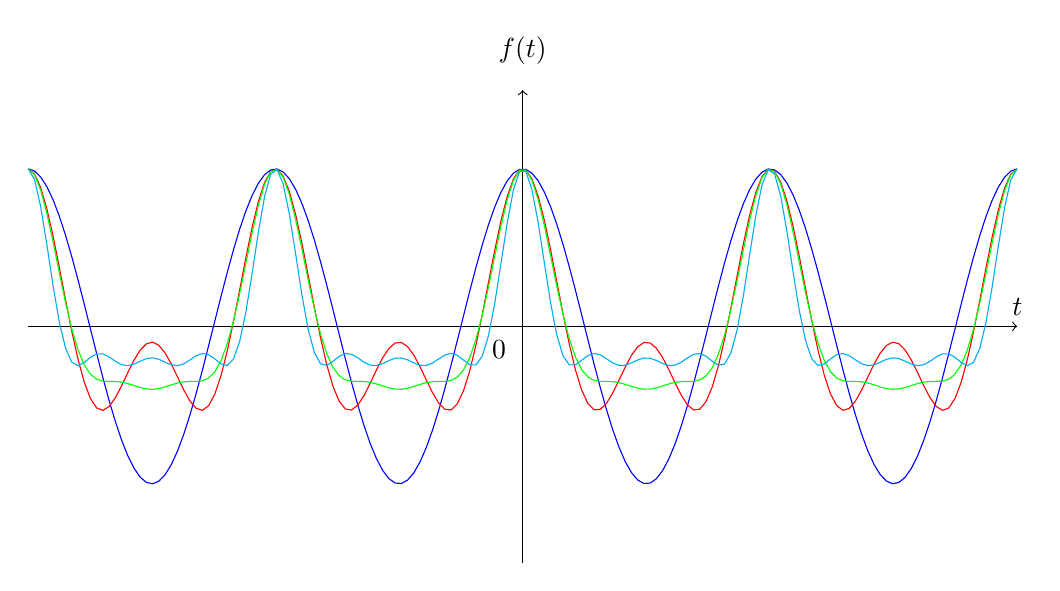
\begin{tikzpicture}

	\draw[->] (-6.28,0)-- (6.28,0);
\draw (-0.3,-0.3) node {0};
\draw[->] (0,-3)-- (0,3);
\draw (2*pi,0.25) node {$t$};
\draw (0,3.5) node {$f(t)$};
%\draw (4.5,-0.3) node {1};

%\draw[thick,blue] (0,0)-- (2.5,0);
%\draw[thick,blue] (2.5,0)-- (4.5,2);
%\draw[thick,blue] (2.5,2)-- (5,2);
\draw[domain=-6.28:6.28,color=blue,samples=160] plot (\x,{2*cos(2*\x r)});
	
	\draw[domain=-6.28:6.28,color=red,samples=160] plot (\x,{2*(0.55*cos(2*\x r)+ 0.45*cos(2*2*\x r))});
	
	\draw[domain=-6.28:6.28,color=green,samples=160] plot (\x,{2*(0.6*cos(2*\x r)+ 0.3*cos(2*2*\x r)+0.1*cos(2*3*\x r))});

		\draw[domain=-6.28:6.28,color=cyan,samples=160] plot (\x,{2*(0.4*cos(2*\x r)+ 0.3*cos(2*2*\x r)+0.2*cos(2*3*\x r) +0.1*cos(2*4*\x r) )});

	\end{tikzpicture}
\end{center}

On a représenté graphiquement les quatre fonctions précédentes dans la figure ci-dessus. On va maintenant représenter les coefficients de leur série de Fourier dans un graphique comprenant la fréquence de l'harmonique en abscisses et son amplitude en ordonnée.

\begin{center}
\begin{tikzpicture}

	\draw[->] (0,0)-- (5,0);
\draw (-0.3,-0.3) node {0};
\draw[->] (0,0)-- (0,3);
\draw (5.1,0.25) node {$f$};
\draw (0,3.5) node {$a_n(f)$};
%\draw (4.5,-0.3) node {1};

\draw[thick,blue] (1,0)-- (1,2);
\draw (1.1,-0.4) node {$\frac{1}{\pi}$};

\draw[thick,red] (1.05,0)-- (1.05,2.5*0.55);
\draw[thick,red] (2.05,0)-- (2.05,2.5*0.45);
\draw (2.1,-0.4) node {$\frac{2}{\pi}$};

\draw[thick,green] (1.1,0)-- (1.1,2.5*0.6);
\draw[thick,green] (2.1,0)-- (2.1,2.5*0.3);
\draw[thick,green] (3.1,0)-- (3.1,2.5*0.1);
\draw (3.1,-0.4) node {$\frac{3}{\pi}$};

\draw[thick,cyan] (1.15,0)-- (1.15,2.5*0.4);
\draw[thick,cyan] (2.15,0)-- (2.15,2.5*0.3);
\draw[thick,cyan] (3.15,0)-- (3.15,2.5*0.2);
\draw[thick,cyan] (4.15,0)-- (4.15,2.5*0.1);
\draw (4.1,-0.4) node {$\frac{4}{\pi}$};

	\end{tikzpicture}
\end{center}

Un premier point important est qu'on a construit des signaux uniquement autour de fonctions cosinus. On peut donc spécifier intégralement le signal en ne traçant que les coefficients $a_n(f)$, mais dans le cas général, il faudrait également tracer les coefficients $b_n(f)$, qui sont ici tous nuls.\\

On note que puisqu'on a utilisé uniquement des cosinus dans la construction du signal, tous les signaux sont "en phase" au sens où les maxima de chaque composantes vont se superposer, ce qui se voit notamment autour de zéro.\\

C'est ce principe de synthèse qui est parfois utilisé dans les générateurs de fonctions en électronique.\\

Une dernière chose importante: La représentation graphique ici ne sera pas qualifié de spectre. Ce terme renvoie à un objet mathématiques bien défini et bien que le lien conceptuel soit assez intuitif, on ne peut rigoureusement parler de spectre pour le graphique précédent.\\

\subsubsection{Transformée de Fourier}

\textbf{Question: Quelle est pour vous le lien entre transformée de Laplace et transformée de Fourier}

Puisqu'on a défini auparavant la transformée de Laplace on peut définir la transformée de Fourier en se basant sur cette dernière. On rappelle la définition de la transformée de Laplace :

\[L{g}(p) = \int^{\infty}_{-\infty} g(t) e^{-pt} \; dt\]\\ 

On peut alors définir la transformée de Fourier de la manière suivante:

\[TF{g}(\omega) = \int^{\infty}_{-\infty} g(t) e^{-j\omega t} \; dt\]\\

On remplace alors la variable de Laplace, $p$ par  $j \omega = 2 \pi j f$ où $f$  est la fréquence qui est homogène à l'inverse d'un temps.\\

La différence entre Fourier et Laplace se situe surtout au niveau du type  d'analyse effectuée. La méthode de Fourier est généralement plus restrictive du fait de sa forme mathématique. Celle-ci se prête notamment mieux aux analyses harmoniques.\\

On peut notamment en avoir l'intuition si on regarde la fonction qui sert à "projeter" le signal $g(t)$ dans l'espace dual. Dans le cas de Laplace, la fonction $e^{-pt}$ peut se décomposer comme $e^{-at}e^{-jbt}$. Le terme de droite est une fonction exponentielle décroissante de la variable temporelle et le membre de gauche est une exponentielle complexe qui peut se réécrire comme une fonction sinusoïdale. Ce qui veut dire que dans le cas de la transformée de Fourier (qui ne conserve que le terme de gauche) l'analyse sera "tournée vers" les fonctions de ce type, et c'est pour cette raison que la transformée de Fourier est un des outils de base de l'analyse harmonique. \\

\textbf{Question: Quelle est pour vous le lien entre les séries de Fourier et transformée de Fourier?} \\

Dans la partie précédente, on a introduit les séries de Fourier et on a construit un graphique où on reportait les coefficients de chaque harmonique. Cela dit, il a été très clairement spécifié que cet outil s'appliquait UNIQUEMENT aux fonctions périodiques. Cette restriction théorique complique l'application des séries de Fourier et l'analyse des harmoniques à beaucoup de signaux "physiques".\\

Sur un plan conceptuel, la transformée de Fourier est une généralisation aux fonctions non-périodiques du développement en série de Fourier. Pour mieux comprendre comment cette généralisation et ses implications on va reprendre l'exemple de nos quatre sommes de cosinus.\\

\textbf{Calculer la transformée de Fourier des quatre fonctions suivantes:}
\begin{enumerate}
\item $g_1(t) = \cos(2 t)$
\item $g_2(t) = 0.55 \cos(2 t) + 0.45 \cos(4 t)$
\item $g_3(t) = 0.6 \cos(2 t) + 0.3 \cos(4 t) + 0.1 \cos(6 t)$
\item $g_4(t) = 0.4 \cos(2 t) + 0.3 \cos(4 t) + 0.2 \cos(6 t) + 0.1 \cos(8 t) $
\end{enumerate} 
On rappelle que la période de toutes ces fonctions est $\pi$

\paragraph{1. $f_1(t) = \cos(2 t)$}
 \[TF{g_1}(f) = \int^{\infty}_{-\infty} g_1(t) e^{-2\pi j f t} \; dt\]
 \[TF{g_1}(f) = \int^{\infty}_{-\infty} \cos(2 t) e^{-2\pi j f t} \; dt\]
\[TF{g_1}(f) = \int^{\infty}_{-\infty} (\frac{e^{2jt} +  e^{-2jt}}{2}) e^{-2\pi j f t} \; dt\]
\[TF{g_1}(f) = \int^{\infty}_{-\infty} (\frac{e^{-j(2 \pi f -2)t}}{2}) \; dt + \int^{\infty}_{-\infty} (\frac{e^{-j(2 \pi f +2)t}}{2}) \; dt\]

pour aller plus loin il faut savoir que : 

 \[\int^{\infty}_{-\infty}  e^{-2\pi j f t} \; dt = \delta(f)\]
 
Ce qui mène à :

\[TF{g_1}(f) = \frac{1}{2}(\delta(f+2) + \delta(f-2))\]

\paragraph{2. $g_2(t) = 0.55 \cos(2 t) + 0.45 \cos(4 t)$}
En repartant du résultat précédent on en déduit le résultat suivant:

\[TF{g_2}(f) = \frac{0.55}{2}(\delta(f+2) + \delta(f-2)) + \frac{0.45}{2}(\delta(f+4) + \delta(f-4))\]

On a donc la somme de 4 diracs, 2 par composantes.

\paragraph{3. $g_3(t) = 0.6 \cos(2 t) + 0.3 \cos(4 t) + 0.1 \cos(6 t)$}
En repartant du résultat précédent on en déduit le résultat suivant:

\[TF{g_3}(f) = \frac{0.6}{2}(\delta(f+2) + \delta(f-2)) + \frac{0.3}{2}(\delta(f+4) + \delta(f-4)) + \frac{0.1}{2}(\delta(f+6) + \delta(f-6))\]

\paragraph{4. $g_4(t) = 0.4 \cos(2 t) + 0.3 \cos(4 t) + 0.2 \cos(6 t) + 0.1 \cos(8 t)$}
En repartant du résultat précédent on en déduit le résultat suivant:

\[TF{g_4}(f) = \frac{0.4}{2}(\delta(f+2) + \delta(f-2)) + \frac{0.3}{2}(\delta(f+4) + \delta(f-4)) + \frac{0.2}{2}(\delta(f+6) + \delta(f-6))\]
\[ + \frac{0.1}{2}(\delta(f+8) + \delta(f-8)) \]


On peut alors tracer le \textbf{spectre} de ces fonctions. Le spectre d'un signal est toujours représenté par deux graphes. Le premier, et celui qu'on se figure plus fréquemment quand on parle de spectre est le spectre en amplitude du signal, qui équivaut au module de la transformée de Fourier du signal.\\

\underline{\textbf{Rappel:}} Soit un complexe $z$ = $a + ib$, alors le module de $z$ est un réel $\rho$ défini comme :

\[ \rho = \sqrt{a^2 + b^2}  \]

On définit également l'argument de $z$ est un réel $\theta$ défini comme:

\[ \theta =  \arctan\frac{b}{a} = \arccos{\frac{a}{\rho}} = \arcsin{\frac{b}{\rho}} \] 

On peut alors écrire le complexe $z$ sous la forme $\rho e^{i \theta}$\\s

Donc si on trace le module du spectre de nos fonctions sinusoïdales précédentes, on obtient le spectre suivant. On note quand dans le cas de la  transformée de Fourier le spectre comporte des composantes positives ET négatives en fréquences ce qui n'était pas le cas dans le représentation en série de Fourier. 
\begin{center}
\begin{tikzpicture}

	\draw[->] (-5,0)-- (5,0);
\draw (-0,-0.3) node {0};
\draw[->] (0,0)-- (0,3);
\draw (5.1,0.25) node {$f$};
\draw (0,3.5) node {$|S(f)|$};
%\draw (4.5,-0.3) node {1};

\draw[thick,blue] (1,0)-- (1,2);
\draw (1.1,-0.4) node {$\frac{1}{\pi}$};

\draw[thick,red] (1.05,0)-- (1.05,2.5*0.55);
\draw[thick,red] (2.05,0)-- (2.05,2.5*0.45);
\draw (2.1,-0.4) node {$\frac{2}{\pi}$};

\draw[thick,green] (1.1,0)-- (1.1,2.5*0.6);
\draw[thick,green] (2.1,0)-- (2.1,2.5*0.3);
\draw[thick,green] (3.1,0)-- (3.1,2.5*0.1);
\draw (3.1,-0.4) node {$\frac{3}{\pi}$};

\draw[thick,cyan] (1.15,0)-- (1.15,2.5*0.4);
\draw[thick,cyan] (2.15,0)-- (2.15,2.5*0.3);
\draw[thick,cyan] (3.15,0)-- (3.15,2.5*0.2);
\draw[thick,cyan] (4.15,0)-- (4.15,2.5*0.1);
\draw (4.1,-0.4) node {$\frac{4}{\pi}$};

\draw[thick,blue] (-1,0)-- (-1,2);
\draw (-1.1,-0.4) node {$\frac{1}{\pi}$};

\draw[thick,red] (-1.05,0)-- (-1.05,2.5*0.55);
\draw[thick,red] (-2.05,0)-- (-2.05,2.5*0.45);
\draw (-2.1,-0.4) node {$\frac{2}{\pi}$};

\draw[thick,green] (-1.1,0)-- (-1.1,2.5*0.6);
\draw[thick,green] (-2.1,0)-- (-2.1,2.5*0.3);
\draw[thick,green] (-3.1,0)-- (-3.1,2.5*0.1);
\draw (-3.1,-0.4) node {$\frac{3}{\pi}$};

\draw[thick,cyan] (-1.15,0)-- (-1.15,2.5*0.4);
\draw[thick,cyan] (-2.15,0)-- (-2.15,2.5*0.3);
\draw[thick,cyan] (-3.15,0)-- (-3.15,2.5*0.2);
\draw[thick,cyan] (-4.15,0)-- (-4.15,2.5*0.1);
\draw (-4.1,-0.4) node {$\frac{4}{\pi}$};

	\end{tikzpicture}
\end{center}

Ici on a représenté le module du spectre mais pas son argument. On a donc un spectre d'amplitude mais pas un spectre de phase or ces deux aspects sont importants dans la représentation d'un signal c'est pourquoi on doit se pencher sur un second exemple pour pouvoir mettre en évidence cette notion de phase.\\

On va donc partir d'un second signal :

\[ g_5(t) = 0.55b\cos(2 t) + 0.45 \cos(4 t + \frac{\pi}{3}) \] 

Il s'agit de la fonction $g_2(t)$ mais légèrement modifiée. On a introduit un déphasage de $\frac{\pi}{3}$. On peut visualiser ce déphasage dans la figure où on a représenté les fonctions $g_2(t)$ et $g_5(t)$.


\begin{center}
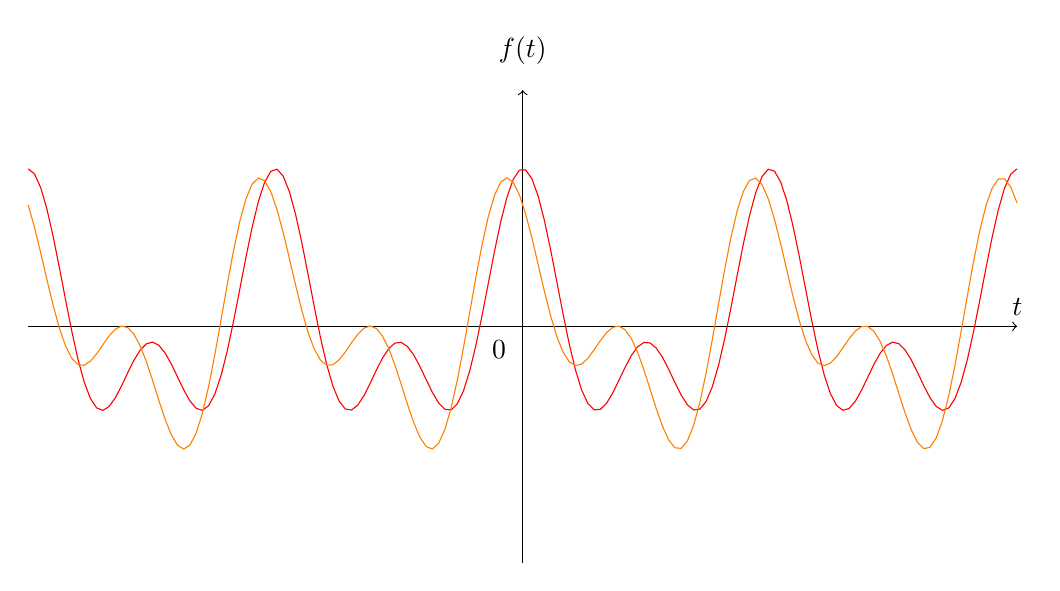
\begin{tikzpicture}

	\draw[->] (-6.28,0)-- (6.28,0);
\draw (-0.3,-0.3) node {0};
\draw[->] (0,-3)-- (0,3);
\draw (2*pi,0.25) node {$t$};
\draw (0,3.5) node {$f(t)$};
%\draw (4.5,-0.3) node {1};

%\draw[thick,blue] (0,0)-- (2.5,0);
%\draw[thick,blue] (2.5,0)-- (4.5,2);
%\draw[thick,blue] (2.5,2)-- (5,2);
	\draw[domain=-6.28:6.28,color=red,samples=160] plot (\x,{2*(0.55*cos(2*\x r)+ 0.45*cos(2*2*\x r))});
	
		\draw[domain=-6.28:6.28,color=orange,samples=160] plot (\x,{2*(0.55*cos(2*\x r)+ 0.45*cos(2*2*(\x+3.14/12) r))});
	
	\end{tikzpicture}
\end{center}
On voit que l'ajout du terme de déphasage a un impact visible sur la forme de la fonction et que le déphasage de la composante "haute fréquence" change la forme du signal.\\

On rappelle la transformée de Fourier du signal précédent :

\[ TF{g_2}(f) =   \frac{0.55}{2}(\delta(f+2) + \delta(f-2)) + \frac{0.45}{2}(\delta(f+4) + \delta(f-4))\]

On peut alors en déduire facilement la transformée de Fourier de $g_5(t)$

\[ TF{g_5}(f) =   \frac{0.55}{2}(\delta(f+2) + \delta(f-2)) + \frac{0.45}{2}(\delta(f+4) + \delta(f-4))e^{-2 j \pi \frac{pi}{3} f }\]

Si $TF{g_2}(f)$ était une fonction réelle (pas de partie complexe), $TF{g_5}(f)$ a clairement une partie imaginaire non nulle. On note également que dans ce cas le module et l'argument sont déjà présentées de façon évidente.\\

Le module des deux fonctions est identique. En effet, on sait que $|e^{-2 j \pi \frac{pi}{3} f }|=1$. Et donc, les modules des deux fonctions sont identiques. Ce qui distingue les deux fonctions dans ce cas est leur phase, soit l'argument de la transformée de Fourier. 

On peut utiliser MATLAB ou GNU/Octave pour représenter les modules de ces fonctions. Ceci sera l'objet d'une de nos activités en salle info



\begin{center}
\begin{tikzpicture}

	\draw[->] (-5,0)-- (5,0);
\draw (-0.3,-0.3) node {0};
\draw[->] (0,-3)-- (0,3);
\draw (5.1,0.25) node {$f$};
\draw (0,3.5) node {$arg(S(f))$};
%\draw (4.5,-0.3) node {1};

\draw[thick,red] (-5,0)-- (5,0);

\draw[thick,orange] (-4.9,3.23)-- (4.9,-3.23);
	\end{tikzpicture}
\end{center}

Cette exemple démontre bien l'importance générale de la phase des signaux et pas seulement de leur spectre d'amplitude qui est souvent ce que les étudiants gardent à l'esprit lorsqu'on leur présente ces notions. Cette notion de phase reprendra de l'importance plus tard lorsqu'on présentera certains types de filtres.

\subsection{Signaux numériques}

\textbf{Question: En quoi consiste la numérisation d'un signal ?} \\

La numérisation d'un signal analogique initial est constitué de deux parties: L'échantillonnage et le codage. Les deux prochaines sous-parties traiteront de chacune de ces notions.

\subsubsection{Codage}

\textbf{Question: Que vous évoque la notion de codage ?} \\

Le codage consiste à \textbf{quantifier} le signal avec une \textbf{dynamique} donnée. Un exemple simple est celui d'une fonction rampe $r(t)$.\\

\begin{center}
\begin{tikzpicture}

	\draw[->] (-4,0)-- (4,0);
\draw (0.3,-0.3) node {0};
\draw[->] (0,-3.2)-- (0,3.2);
\draw (4.1,0.25) node {$t$};
\draw (0,3.5) node {$r(t)$};

\draw (1,-0.1)-- (1,0.1);
\draw (1.0,-0.3) node {1};
\draw (2,-0.1)-- (2,0.1);
\draw (2.0,-0.3) node {2};
\draw (3,-0.1)-- (3,0.1);
\draw (3.0,-0.3) node {3};

\draw (-1,-0.1)-- (-1,0.1);
\draw (-1.0,0.3) node {-1};
\draw (-2,-0.1)-- (-2,0.1);
\draw (-2.0,0.3) node {-2};
\draw (-3,-0.1)-- (-3,0.1);
\draw (-3.0,0.3) node {-3};

\draw (-0.1,1)-- (0.1,1);
\draw (-0.3,1) node {1};
\draw (-0.1,2)-- (0.1,2);
\draw (-0.3,2) node {2};
\draw (-0.1,3)-- (0.1,3);
\draw (-0.3,3) node {3};

\draw (-0.1,-1)-- (0.1,-1);
\draw (0.3,-1) node {-1};
\draw (-0.1,-2)-- (0.1,-2);
\draw (0.3,-2) node {-2};
\draw (-0.1,-3)-- (0.1,-3);
\draw (0.3,-3) node {-3};

%r(t)
\draw[thick,blue] (-3,-3)-- (3,3);

\draw[thick,dashed,red] (-3,-3)-- (-2,-3);
\draw[thick,dashed,red] (-2,-3)-- (-2,-2);
\draw[thick,dashed,red] (-2,-2)-- (-1,-2);
\draw[thick,dashed,red] (-1,-2)-- (-1,-1);
\draw[thick,dashed,red] (-1,-1)-- (-0,-1);
\draw[thick,dashed,red] (-0,-1)-- (-0,-0);
\draw[thick,dashed,red] (-0,-0)-- (1,-0);
\draw[thick,dashed,red] (1,0)-- (1,1);
\draw[thick,dashed,red] (1,1)-- (2,1);
\draw[thick,dashed,red] (2,1)-- (2,2);
\draw[thick,dashed,red] (2,2)-- (3,2);
\draw[thick,dashed,red] (3,2)-- (3,3);

\draw[thick,dashed,green] (-3,-2)-- (-2,-2);
\draw[thick,dashed,green] (-3,-3)-- (-3,-2);
\draw[thick,dashed,green] (-2,-1)-- (-1,-1);
\draw[thick,dashed,green] (-2,-2)-- (-2,-1);
\draw[thick,dashed,green] (-1,-0)-- (-0,-0);
\draw[thick,dashed,green] (-1,-1)-- (-1,0);
\draw[thick,dashed,green] (-0,1)-- (1,1);
\draw[thick,dashed,green] (0,0)-- (0,1);
\draw[thick,dashed,green] (1,2)-- (2,2);
\draw[thick,dashed,green] (1,1)-- (1,2);
\draw[thick,dashed,green] (2,3)-- (3,3);
\draw[thick,dashed,green] (2,2)-- (2,3);
	\end{tikzpicture}
\end{center}

On voit dans la figure précédente deux exemples de quantification de la fonction rampe avec une \textbf{amplitude de crête} de 3 unités et un \textbf{échelon de quantification} d'une unité Dans un cas, on échantillonne par arrondi (vert) et dans l'autre on arrondit par troncature (rouge). On peut aussi imaginer un cas intermédiaire où la valeur de quantification correspondrait au milieu de l'intervalle.\\

Généralement, le codage se fait sur des nombres binaires. le nombre de valeurs disponibles est alors généralement donné par le nombre de bit utilisé pour le codage.\\

\textbf{Exercice: Si on code un signal d'une amplitude de crête de 5 volts sur 4 bits, quelle est la valeur de l'échelon de quantification ?}

4 bits binaires permettent de représenter 16 valeurs. L'intervalle [-5; 5] couvre 10 V au total. La solution la plus directe est de diviser la gamme en 10 secteurs égaux et de faire correspondre une des 16 valeurs binaires à chacun. Les secteurs ont une étendue de 0.625 V chacun et on peut diviser la gamme en 2N secteurs.

\begin{table}[h!]
\begin{center}
\begin{tabular}{|p{20mm}|p{10mm}|p{25mm}|}
 \hline
 code binaire &  valeur & amplitude \\
 \hline
 0000 & 0 &  [-5.000;-4.375] \\
 \hline
 0001 & 1 & [-4.375; -3.750]\\
 \hline
 0010 & 2 & [-3.750;-3.125]\\
 \hline
 0011 & 3 & [-3.125;-2.500]\\
 \hline
 0100 & 4 & [-2.500;-1.875]\\
 \hline
 0101 & 5 & [-1.875;-1.250]\\
 \hline
 0110 & 6 & [-1.250;-0.625]\\
 \hline
 0111 & 7 & [-0.625;0.000]\\
 \hline
 1000 & 8 &  [0.000;0.625]\\
 \hline
 1001 & 9 &  [0.625;1.250]\\
 \hline
 1010 & 10 & [1.250;1.875]\\
 \hline
 1011 & 11 & [1.875;2.500]\\
 \hline
 1100 & 12 & [2.500;3.125]\\
 \hline
 1101 & 13 & [3.125;3.750]\\
 \hline
 1110 & 14 & [3.750;4.375]\\
 \hline
 1111 & 15 & [4.375;5.000]\\
 \hline 
\end{tabular}
\end{center}
\end{table}

Le principe présenté dans la figure précédente s'applique de nouveau ici puisque chaque intervalle ne correspondra qu'à une valeur finale qui peut être sa borne inférieure, sa borne supérieure, ou une valeur intermédiaire. Mais il est important de comprendre qu'à ce stade on a aucun moyen de connaître la valeur plus précisément que ce que permet l'échelon de quantification.\\


L'approximation systématique du au codage induit une erreur et donc un bruit de quantification. Ce bruit de quantification dépend donc de paramètres très important du processus de codage. L'amplitude de codage, et l'échelon de quantification.\\

\subsubsection{L'échantillonnage}

\textbf{Question : En quoi consiste pour vous l'opération d'échantillonnage ?}

D'après le livre de Maurice Bellanger : "L’échantillonnage consiste à représenter un signal fonction du temps $s(t)$ par ses
valeurs $s(nT_e)$ à des instants multiples entiers d’une durée $T_e$, appelée période d’échantillonnage."\\

Mathématiquement, l'opération d'échantillonnage s'appuie sur la distribution appelée "peigne de Dirac" et qui est définie comme suit: 

\[ u_{T_e}(t) = \sum_{n = -\infty}^{\infty} \delta(t-nT_e) \]\\

Le signal échantillonné avec une période $T_e$ peut alors s'exprimer comme le produit $u_{T_e}(t) s(t)$.\\

\begin{center}
\begin{tikzpicture}

	\draw[->] (-5,0)-- (5,0);
\draw (-0.3,-0.3) node {0};
\draw[->] (0,-3)-- (0,3);
\draw (5.1,0.25) node {$f$};
\draw (0,3.5) node {$s(t)$};
%\draw (4.5,-0.3) node {1};

\draw[domain=-4.9:4.9,color=blue,samples=160] plot (\x,{2*(0.55*cos(2*\x r)+ 0.45*cos(2*2*(\x+3.14/12) r))});
	\end{tikzpicture}
\end{center}

\begin{center}
\begin{tikzpicture}

	\draw[->] (-5,0)-- (5,0);
\draw (-0.3,-0.3) node {0};
\draw[->] (0,-3)-- (0,3);
\draw (5.1,0.25) node {$f$};
\draw (0,3.5) node {$u_{T_e}(t)$};
%\draw (4.5,-0.3) node {1};

\draw[thick,blue] (-4,-0)-- (-4,1);
\draw[thick,blue] (-3,-0)-- (-3,1);
\draw[thick,blue] (-2,-0)-- (-2,1);
\draw[thick,blue] (-1,-0)-- (-1,1);
\draw[thick,blue] (0,-0)-- (0,1);
\draw[thick,blue] (1,-0)-- (1,1);
\draw[thick,blue] (2,-0)-- (2,1);
\draw[thick,blue] (3,-0)-- (3,1);
\draw[thick,blue] (4,-0)-- (4,1);
	\end{tikzpicture}
\end{center}

\begin{center}
\begin{tikzpicture}

	\draw[->] (-5,0)-- (5,0);
\draw (-0.3,-0.3) node {0};
\draw[->] (0,-3)-- (0,3);
\draw (5.1,0.25) node {$f$};
\draw (0,3.5) node {$u_{T_{e}}(t)s(t)$};
%\draw (4.5,-0.3) node {1};

\draw[dashed,domain=-4.9:4.9,color=blue,samples=160] plot (\x,{2*(0.55*cos(2*\x r)+ 0.45*cos(2*2*(\x+3.14/12) r))});

\draw[thick,blue] (-4,-0)-- (-4,-0.9);
\draw[thick,blue] (-3,-0)-- (-3,1);
\draw[thick,blue] (-2,-0)-- (-2,0);
\draw[thick,blue] (-1,-0)-- (-1,-1.25);
\draw[thick,blue] (0,-0)-- (0,1.3);
\draw[thick,blue] (1,-0)-- (1,-0.15);
\draw[thick,blue] (2,-0)-- (2,-1.5);
\draw[thick,blue] (3,-0)-- (3,1.8);
\draw[thick,blue] (4,-0)-- (4,-0.35);
	\end{tikzpicture}
\end{center}

Une des premières choses à aborder dans ce cas est l'impact de l'opération d'échantillonnage sur le spectre du signal:\\

\[ TF (\sum_{n = -\infty}^{\infty} s(t)\delta(t-nT_e)) = \sum_{n = -\infty}^{\infty} TF(s(t)\delta(t-nT_e) ) \]

\[ \sum_{n = -\infty}^{\infty} TF(s(t)\delta(t-nT_e) ) = \sum_{n = -\infty}^{\infty} S(f) \star e^{- 2j\pi n T_e f} \]\\

Pour aller plus loin il faut savoir que : 

\[ \sum_{n = -\infty}^{\infty} e^{- 2j\pi n T_e f} = \frac{1}{T_e} \sum_{n = -\infty}^{\infty} \delta(f - \frac{n}{T}) \]\\

Et que 

\[\delta \star \phi = \phi \]

Ce qui mène à 

\[ TF (\sum_{n = -\infty}^{\infty} s(t)\delta(t-nT_e)) = \frac{1}{T}\sum_{n = -\infty}^{\infty} S(f) \star \delta(f - \frac{n}{T_e})\]

La dernière expression traduit le fait que le spectre se répète dans l'espace des fréquences avec une période de $\frac{1}{T_e}$.\\

On va continuer avec l'exemple de la fonction $ g_5(t) = \cos(2 t) + 0.45 \cos(4 t + \frac{\pi}{3})$ dont on retrace le module du spectre dans  la figure suivante.

\begin{center}
\begin{tikzpicture}

	\draw[->] (-5,0)-- (5,0);
\draw (-0,-0.3) node {0};
\draw[->] (0,0)-- (0,3);
\draw (5.1,0.25) node {$f$};
\draw (0,3.5) node {$|S(f)|$};
%\draw (4.5,-0.3) node {1};


\draw[thick,blue] (1.05,0)-- (1.05,2.5*0.55);
\draw[thick,blue] (2.05,0)-- (2.05,2.5*0.45);
\draw (2.1,-0.4) node {$\frac{2}{\pi}$};
\draw (1.1,-0.4) node {$\frac{1}{\pi}$};

\draw[thick,blue] (-1.05,0)-- (-1.05,2.5*0.55);
\draw[thick,blue] (-2.05,0)-- (-2.05,2.5*0.45);
\draw (-2.1,-0.4) node {$\frac{2}{\pi}$};
\draw (-1.1,-0.4) node {$\frac{1}{\pi}$};


	\end{tikzpicture}
\end{center}

\textbf{Question: Que doit-on avoir à l'esprit  lors du choix de la période d’échantillonnage ?}\\

Lors de l'échantillonnage, on doit conserver l'information, mais aussi optimiser la quantité de données à gérer dans la plupart des cas.\\

Le théorème de Nyquist-Shannon dit : \textbf{"La représentation discrète d'un signal exige des échantillons régulièrement espacés à une fréquence d'échantillonnage supérieure au double de la fréquence maximale présente dans ce signal."}\\

Visuellement, il faut se figurer que la fréquence la plus élevée dans la norme du spectre donne la largeur du spectre. Dans le domaine temporel, cela se comprend de la façon suivante la variation avec la plus petite échelle temporelle n'est conservée que si la période d'échantillonnage permet d'en isoler au moins 2 points.\\

Lors de l'échantillonnage, le spectre est répliqué avec sa largeur complète à TOUS les multiples de la fréquence d'échantillonnage.\\

\textbf{Question: Quelle est la gamme de fréquences d'échantillonnage garantissant le respect de Nyquist-Shannon pour le signal $g5(t)$?}\\

Dans le cas de la fonction $g_5(t) = \cos(2 t) + 0.45 \cos(4 t + \frac{\pi}{3})$, on a vu dans la figure précédente que le spectre en amplitude présente deux raies. la fréquence maximale correspond donc à celle de la 2e raie : $\frac{2}{\pi}$. Le double de cette fréquence maximale donne donc $f_e = \frac{4}{\pi}$, et donc une période de $\frac{\pi}{4}$\\

\begin{center}
\begin{tikzpicture}

	\draw[->] (-5,0)-- (5,0);
\draw (-0.3,-0.3) node {0};
\draw[->] (0,-3)-- (0,3);
\draw (5.1,0.25) node {$f$};
\draw (0,3.5) node {$u_{T_{e}}(t)s(t)$};
%\draw (4.5,-0.3) node {1};

\draw[dotted,domain=-4.9:4.9,color=blue,samples=160] plot (\x,{2*(0.55*cos(2*\x r)+ 0.45*cos(2*2*(\x+3.14/12) r))});

\draw[thick,blue] (-4.74,-0)-- (-4.74,-0.55);
\draw[thick,blue] (-3.95,-0)-- (-3.95,-0.60);
\draw[thick,blue] (-3.16,-0)-- (-3.16,1.6);
\draw[thick,blue] (-2.37,-0)-- (-2.37,-0.45);
\draw[thick,blue] (-1.58,-0)-- (-1.58,-0.65);
\draw[thick,blue] (-0.79,-0)-- (-0.79,-0.65);
\draw[thick,blue] (0,-0)-- (0,1.5);
\draw[thick,blue] (0.79,-0)-- (0.79,-0.45);
\draw[thick,blue] (1.58,-0)-- (1.58,-0.6);
\draw[thick,blue] (2.37,-0)-- (2.37,-0.25);
\draw[thick,blue] (3.16,-0)-- (3.16,1.55);
\draw[thick,blue] (3.95,-0)-- (3.95,-0.45);
\draw[thick,blue] (4.74,-0)-- (4.74,-0.7);

\draw[dashed,cyan] (-4.74,-0.55)-- (-3.95,-0.6)--(-3.95,-0.6)--(-3.16,1.6)--(-2.37,-0.45)--(-1.58,-0.65)--(-0.79,-0.65)--(0,1.5)--(0.79,-0.45)--(1.58,-0.6)--(2.37,-0.25)--(3.16,1.55)--(3.95,-0.45)--(4.74,-0.7);

	\end{tikzpicture}
\end{center}

On voit bien si on représente la fonction échantillonnée que le respect strict ou minimal de la condition de Nyquist-Shannon donne lieu à une reconstruction qui peut paraître assez éloignée de la fonction initiale.  
\\

On peut également représenter le spectre en amplitude du signal échantillonnée. On rappelle que l'échantillonnage à une fréquence consiste à périodiser le spectre en fréquence avec une période de $f_e$. On va donc représenter ce spectre en amplitude dans la figure suivante.\\

\begin{center}
\begin{tikzpicture}

	\draw[->] (-7,0)-- (7,0);
\draw (-0,-0.3) node {0};
\draw[->] (0,0)-- (0,3);
\draw (7.1,0.25) node {$f$};
\draw (0,3.5) node {$|S(f)|$};
%\draw (4.5,-0.3) node {1};


\draw[thick,blue] (1.05,0)-- (1.05,2.5*0.55);
\draw[thick,blue] (2.05,0)-- (2.05,2.5*0.45);
\draw (2.1,-0.4) node {$\frac{2}{\pi}$};
\draw (1.1,-0.4) node {$\frac{1}{\pi}$};

\draw[thick,blue] (-1.05,0)-- (-1.05,2.5*0.55);
\draw[thick,blue] (-2.05,0)-- (-2.05,2.5*0.45);
\draw (-2.1,-0.4) node {$-\frac{2}{\pi}$};
\draw (-1.1,-0.4) node {$-\frac{1}{\pi}$};


%replica 1
\draw[thick,cyan] (5.05,0)-- (5.05,2.5*0.55);
\draw[thick,cyan] (6.05,0)-- (6.05,2.5*0.45);
\draw (5.1,-0.4) node {$\frac{5}{\pi}$};
\draw (6.1,-0.4) node {$\frac{6}{\pi}$};

\draw[thick,cyan] (3.05,0)-- (3.05,2.5*0.55);
\draw[thick,cyan] (2.08,0)-- (2.08,2.5*0.45);
\draw (3.1,-0.4) node {$\frac{3}{\pi}$};
%\draw (2.1,-0.4) node {$\frac{1}{\pi}$};
\draw (4.1,-0.4) node {$\frac{4}{\pi}$};


%replica 2
\draw[thick,cyan] (-5.05,0)-- (-5.05,2.5*0.55);
\draw[thick,cyan] (-6.05,0)-- (-6.05,2.5*0.45);
\draw (-5.1,-0.4) node {$-\frac{5}{\pi}$};
\draw (-6.1,-0.4) node {$-\frac{6}{\pi}$};

\draw[thick,cyan] (-3.05,0)-- (-3.05,2.5*0.55);
\draw[thick,cyan] (-2.08,0)-- (-2.08,2.5*0.45);
\draw (-3.1,-0.4) node {$-\frac{3}{\pi}$};
%\draw (2.1,-0.4) node {$\frac{1}{\pi}$};
\draw (-4.1,-0.4) node {$-\frac{4}{\pi}$};


	\end{tikzpicture}
\end{center}

Le spectre en amplitude permet de comprendre la notion de \textbf{repliement spectral}. Si on respecte le théorème de Nyquist-Shannon strictement on voit que les extrémités des répliques dues à l'échantillonnage sont quasiment confondues. Et donc si on choisit une fréquence d'échantillonnage inférieure, on va se retrouver avec des spectres qui se mélangent. Dans le domaine temporel cela va évidemment correspondre à des échantillons ne permettant pas de capturer toutes les caractéristiques du signal.\\

\subsubsection{Propriétés des signaux échantillonnés: Cas usuels}
% Kronecker
% signal échelon 
% etc...

\subsection{La transformée en Z}
Une outil mathématique particulièrement important en traitement du signal/filtrage numérique est la transformée en Z .\\

\textbf{Question: Que vous évoque la notion de transformée en Z ?}\\

La transformée en Z est définie de la façon suivante :

\[\sum_{n = 0}^{\infty} s_{T_e}(n) z^{-n}\] 

On la compare généralement à la transformée de Laplace. L'intégrale (somme continue) est remplacée par une somme discrète, et le terme exponentiel est remplacé par $z^{-n}$ C'est ce terme qui donne son nom à la transformée en Z. Tout comme $p$ dans la transformée de Laplace, $z$  est une variable \textbf{complexe}. Il est important de noter que le fait que la somme soit infinie oblige la variable $z$ à avoir un module inférieur à 1 pour converger.\\

La comparaison avec la transformée de Laplace vient surtout du fait que la transformée en Z a des propriétés sur des signaux discrets très similaires à celle de la transformée de Laplace pour les signaux continus. C'est ce qu'on va illustrer dans les sous-parties suivantes.\\

\subsubsection{Transformée en Z des fonctions usuelles}

\textbf{Exercice: Calculez les transformées en Z des quatre suites suivantes}
\begin{enumerate}
\item $\delta[n]$
\item $u[n]$
\item $nu[n]$
\item $sin(\omega_0 n)u(n)$
\end{enumerate} 

\textbf{1. $\delta[n]$}
\[\sum_{n = 0}^{\infty} \delta[n] z^{-n}\] \\

$\delta[n]$ est la suite définie comme prenant la valeur 1 pour l'échantillon d'index 0 et 0 sur tous les autres points. Donc,\\

\[\sum_{n = 0}^{\infty} \delta[n] z^{-n} = z^0 = 1 \]\\

\textbf{2. $u[n]$}

$u[n]$ est la suite définie comme prenant la valeur 1 pour l'échantillon d'index 0 et tous les suivants. Donc,\\

\[\sum_{n = 0}^{\infty} u[n] z^{-n} = \sum_{n = 0}^{\infty} z^{-n}  = \frac{1}{1-z^{-1}} \]\\

La dernière étape est un résultat connu sur la série géométrique convergente. Ce résultat n'est d'ailleurs vraie que si la valeur absolue ou le module de la raison de la suite (ici, $z$) est strictement inférieur à 1.  Dans le cas de l'analyse de Fourier la question ne se pose jamais car $z$ est remplacé par $e^{j\frac{2 \pi k }{N}}$, un nombre complexe qui est toujours de  module 1.\\

Ce résultat est important à la fois du point de vue purement mathématique des suites mais aussi en analyse de stablilité pour les filtres.\\

En effet on rappelle qu'avec l'analyse de  Laplace la variable $p$ est en général décomposée en $p = \sigma + j \omega$.  $\sigma$ décrit alors les régimes transitoires (décroissance exponentielle, etc...) alors que la partie imaginaire $\omega$ est la réponse à une excitation periodique (et donc sinusoïdale)

\textbf{3. $nu[n]$}

 $nu[n]$ est l'équivalent discret de la fonction rampe.\\
 

\[\sum_{n = 0}^{\infty} n u[n] z^{-n} = \sum_{n = 0}^{\infty} n z^{-n}  = \frac{z^{-1}}{(1-z^{-1})^2} \]\\ 

Dans ce cas, la valeur de la somme peut se démontrer en utilisant une méthode analogue au cas précédent mais cette fois dans le cas d'une suite arithmético-géométrique.

%proof : https://en.wikipedia.org/wiki/Arithmetico-geometric_sequence#Sum_of_the_terms


\subsubsection{Propriétés de la transformée en Z}

\textbf{Exercice : démontrer la linéarité de la transformée en Z}\\

soit $x(n) = a x_1(n) + b x_2(n)$, alors,

\[X(z) = \sum_{n = 0}^{\infty} x(n) z^{-n}\] 

\[X(z) = \sum_{n = 0}^{\infty} (a x_1(n) + b x_2(n)) z^{-n}\] 

\[X(z) = a \sum_{n = 0}^{\infty} x_1(n)  z^{-n} + b \sum_{n = 0}^{\infty} x_2(n) \] 

\[X(z) = a X_1(z)+ b X_2(z) \] 

\textbf{Exercice : Calculer la transformée en Z de $x_1(n) \star x_2(n)$}\\

Dans un premier temps il faut établir ce qu'est la convolution  de deux signaux discrets.

\[ x_1(n) \star x_2(n)=  \sum_{k = -\infty}^{\infty} x_1(n-k)x_2(n) \]

Cette définition est analogue à celle de la convolution dans le domaine continu. On peut ensuite appliquer la transformée en Z. La démonstration est simple mais pas forcément intuitive.

\[ TZ(x_1(n) \star x_2(n)) = \sum_{n = -\infty}^{\infty} \sum_{k = -\infty}^{\infty} x_1(n-k)x_2(n) z^{-n}\]

On peut alors réécrire la variable de la transformée en z sous une autre forme sans changer l'égalité.

\[ TZ(x_1(n) \star x_2(n)) = \sum_{n = -\infty}^{\infty} \sum_{k = -\infty}^{\infty} x_1(n-k)x_2(k) z^{-k}  z^{-(n-k)}\]

Puisque $k$ peut prendre n'importe quelle valeur on peut le réécrire sous la forme d'un entier unique $m$ 

\[ TZ(x_1(n) \star x_2(n)) = \sum_{n = -\infty}^{\infty} \sum_{m = -\infty}^{\infty} x_1(m)x_2(k) z^{-k}  z^{-(m)}\]

On a donc une expression où on peut regrouper les sommes dans deux produits.

\[ TZ(x_1(n) \star x_2(n)) = \sum_{n = -\infty}^{\infty} x_2(k)z^{-k} \sum_{m = -\infty}^{\infty} x_1(m)   z^{-(m)}\]

\[ TZ(x_1(n) \star x_2(n)) = TZ(x_1) TZ(x_2)\]

\subsection{La transformée de Fourier discrète (TFD)}

\textbf{Question: Que vous évoque la notion de transformée de Fourier Discrète ?}\\

Dans la sous-partie précédente on a présenté la transformée en Z. La transformée en Z est un outil "général" permettant l'analyse de système  opérant sur des temps discrets. On peut alors calculer la transformée de Fourier d'un signal discret en faisant le changement de variable suivant : $z = e^{j2\pi f T_e}$ avec $T_e$ la période d'échantillonnage du signal discret. Soit $s[n]$ un signal discret, La transformée de Fourier d'un signal discret s'écrit alors : 

\[ TF\lbrace s \rbrace(f) = S(f) = \sum_{k = 0}^{\infty} s[k] \; e^{-j 2 \pi k f T_e}\] \\

Or cette transformée de Fourier, strictement équivalent à la transformée en z au changement de variable de près jusqu'ici, n'est pas calculable par un ordinateur, ou un système à mémoire finie quelconque.\\

\textbf{Question: Pourquoi ? Et secondement,  comment ce "problème" est-il contourné ?}\\

On doit numériser le signal, mais cela veut dire que si on fait des calculs sur son spectre ce dernier doit également être numérisé, c'est-à-dire échantillonné et codé même si on laissera de côté la question du codage pour l'instant. Donc on repart de la transformée de Fourier $S(f)$ d'un signal discret $s[n]$ :\\

\[ TF\lbrace s \rbrace(f) = S(f) = \sum_{k = 0}^{\infty} s[k] \; e^{-j 2 \pi k f T_e} \rightarrow S^{\star} (f) =  \sum_{k = 0}^{N-1} s[k] \; e^{-j 2 \pi k f T_e} \]\\


\textbf{Question : à ce stade, compte tenu de la problématique initial il manque encore une étape. Laquelle ?}\\

Et oui... Même si le nombre de termes de la somme reste fini la fonction continue au membre de gauche signifie que cette fonction sera continue. On peut d'ailleurs s'en rendre compte avec l'exemple de la fonction rectangle discrétisée. Sa transformée de Fourier n'a pas un nombre infini de terme non nuls et pourtant elle est une fonction continue et contenant donc une infinité de valeurs à représenter. Il faut donc également échantillonner le spectre.\\

\[\sum_{k = 0}^{N-1} s[k] \; e^{-j 2 \pi k f T_e} \rightarrow S^{\star} (m \Delta f) = \sum_{k = 0}^{N-1} s[k] \; e^{-j 2 \pi k m \Delta f T_e} \]\\

à ce stade, il nous faut encore déterminer la valeur de $\Delta f$, l'incrément en fréquence.\\

\textbf{Question : Quelle valeur suggérez-vous et pourquoi ?}\\

Un choix évident, notamment en terme de mémoire est de se dire que si on dispose de $N$ valeurs pour le signal temporel, on va également prendre $N$ valeurs pour le spectre du signal.On rappelle ici que l'échantillonnage d'un signal dans le domaine temporelle conduit à la périodisation de son spectre dans le domaine fréquentiel avec une fréquence $f_e$. On doit donc prendre un nombre discret de valeurs sur un intervalle de fréquence de largeur $f_e$ pour avoir tout le spectre. Donc, $\Delta f = \frac{f_e}{N}$ et\\

\[S^{\star} (m \frac{f_e}{N}) = \sum_{k = 0}^{N-1} s[k] \; e^{-j 2 \pi k m \frac{f_e}{N} T_e} \]\\

On insiste bien ici sur le fait que pour avoir le terme d'indice $m$ de la suite du spectre, il faut sommer $N$ terme de la suite correspondant au signal temporel avec le bon indice $m$ dans le terme exponentiel.\\

Afin de bien illustrer le lien entre toutes les notions evoquées jusqu'ici on va reprendre le cas de la fonction rectangulaire.

\begin{center}
\begin{tikzpicture}

	\draw[->] (-3,0)-- (3,0);
\draw (-0.3,-0.3) node {0};
\draw[->] (0,0)-- (0,1.5);
\draw (3.1,0.25) node {$t$};
\draw (0,2) node {$e(t)$};


\draw[thick,blue](-3,0)--(-1.5,0)--(-1.5,1)--(-1.5,1)--(0,1)--(1.5,1)--(1.5,0)--(3,0);


\draw[->] (3.5,1)-- (4.5,1);

\draw[->] (7.5,0)-- (7.5,1.5);
\draw (7.5,-0.3) node {0};
\draw[->] (5,0)-- (10,0);
\draw (10.1,0.25) node {$f$};
\draw (7.5,2) node {$E(f)$};
\draw[ domain=4.9:9.9,color=blue,samples=160] plot (\x,{80*sin(5*3.14*\x r -5*3.14*7.5r )/(5*3.14*\x r-5*3.14*7.5 r)});


\end{tikzpicture}
\end{center}

La fonction rectangulaire en temporel continu va correspondre à un sinus cardinal continu en fréquence.  
\begin{center}
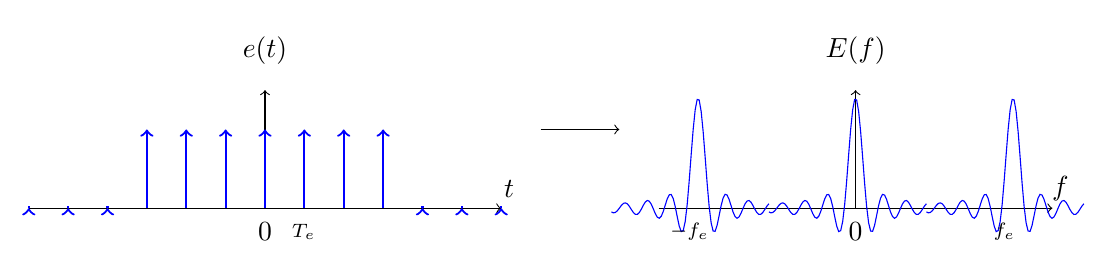
\begin{tikzpicture}

	\draw[->] (-3,0)-- (3,0);
\draw (0,-0.3) node {0};
\draw (0.5,-0.3) node {$_{T_e}$};
\draw[->] (0,0)-- (0,1.5);
\draw (3.1,0.25) node {$t$};
\draw (0,2) node {$e(t)$};

\foreach \x in {-3,-2.5,...,-2} \draw[->,thick,blue](\x,0)--(\x,0);
\foreach \x in {-1.5,-1,...,1.5} \draw[->,thick,blue](\x,0)--(\x,1);
\foreach \x in {2,2.5,...,3} \draw[->,thick,blue](\x,0)--(\x,0);
%\draw[->,thick,blue](-3,0)--(-3,0);

\draw[->] (3.5,1)-- (4.5,1);

\draw[->] (7.5,0)-- (7.5,1.5);
\draw (7.5,-0.3) node {0};
\draw[->] (5,0)-- (10,0);
\draw (10.1,0.25) node {$f$};
\draw (7.5,2) node {$E(f)$};
\draw[ domain=6.4:8.4,color=blue,samples=80] plot (\x,{80*sin(7*3.14*\x r -7*3.14*7.5r )/(7*3.14*\x r-7*3.14*7.5 r)});
\draw[ domain=4.4:6.4,color=blue,samples=80] plot (\x,{80*sin(7*3.14*\x r -7*3.14*5.5r )/(7*3.14*\x r-7*3.14*5.5 r)});
\draw[ domain=8.4:10.4,color=blue,samples=80] plot (\x,{80*sin(7*3.14*\x r -7*3.14*9.5r )/(7*3.14*\x r-7*3.14*9.5 r)});
\draw (5.4,-0.3) node {$_{-f_e}$};
\draw (9.4,-0.3) node {$_{f_e}$};

\end{tikzpicture}
\end{center}

L'échantillonage à période $T_e$ en temporel périodise le spectre avec une période de $f_e$. Mais ça ce stade on a toujours un signal et un spectre infinis.\\ 

Pour passer à un spectre compatible avec un stockage numérique il faut échantillonner et stocker une des périodes. Or on rappelle qu'échantillonner dans un domaine, c'est périodiser dans l'autre.
% combed sinc
%\draw[->] (7.5,0)-- (7.5,1.5);
%\draw (7.5,-0.3) node {0};
%\draw[->] (5,0)-- (10,0);
%\draw (10.1,0.25) node {$f$};
%\draw (7.5,2) node {$e(f)$};
%\draw[ domain=4.9:9.9,color=blue,samples=80] plot[ycomb] (\x,{80*sin(5*3.14*\x r -5*3.14*7.5r )/(5*3.14*\x r-5*3.14*7.5 r)});
%

%fct ech
%\draw[red] (7.5,0)-- (7.5,1.4);
%\draw[red] (7.75,0)-- (7.75,-0.25);
%\draw[red] (7.25,0)-- (7.25,-0.25);
%\draw[red] (8,0)-- (8,0.17);
%\draw[red] (7,0)-- (7,0.17);
%\draw[red] (8.25,0)-- (8.25,-0.1);
%\draw[red] (6.75,0)-- (6.75,-0.1);
%\draw[red] (8.5,0)-- (8.5,0.01);
%\draw[red] (6.5,0)-- (6.5,0.01);
%\draw[red] (8.75,0)-- (8.75,0.07);
%\draw[red] (6.25,0)-- (6.25,0.07);
%\draw[red] (9,0)-- (9,-0.075);
%\draw[red] (6,0)-- (6,-0.075);
%\draw[red] (9.25,0)-- (9.25,0.03);
%\draw[red] (5.75,0)-- (5.75,0.03);
%\draw[red] (9.5,0)-- (9.5,-0.01);
%\draw[red] (5.5,0)-- (5.5,-0.01);
%\draw[red] (9.75,0)-- (9.75,-0.02);
%\draw[red] (5.25,0)-- (5.25,-0.02);

\subsection{Conclusion Rappels}
Dans cette section sur les fondamentaux, on a rappelé des définitions importantes en traitement du signal et on les replacés dans le contexte du traitement du signal numérique et des chaînes d'instrumentation.\\

On a rappelé les notions d'invariance dans le temps et de linéarité des filtres et leur importance dans l'établissement de la relation de convolution.\\

On a rappelé les définitions des transformées de Fourier et de Laplace, leur propriétés ainsi que quelques transformées usuelles par le biais d'exemple.\\

On a ensuite abordé les notions importantes de codage et d'échantillonnage pour passer un signal du domaine temporel continu au domaine temporel discret. On a pu voir l'impact de l'échantillonnage sur le spectre en amplitude et on a rappelé l'importance du théorème de Nyquist-Shannon. \\
pur finir on a discuté des propriétés particulières des signaux échantillonnés et on a les comparés à celles de signaux continus équivalents.\\

\section{Filtres numériques : Généralités}
On rappelle qu'un filtre numérique va lier une entrée $x(n)$ à une sortie $y(n)$. On avait discuté plus tôt l'importance capitale des propriétés de linéarité et de l'invariance dans le temps puisque ces conditions sont des pré-requis au fait que le filtre/système puisse être décrit par sa seule réponse impulsionnelle.\\

\textbf{Question: Rappelez pour une filtre linéaire invariant dans le temps discret l'équation liant l'entrée et la sortie}\\

\[ y(n) = \sum_{m = 0}^{N-1} h(m) x(n-m) \]\\

On rappelle que dans le cadre des systèmes linéaires et invariants dans le temps, $h(m)$ est la réponse impulsionnelle du filtre discret qui le caractérise entièrement.


\subsection{Notion de récursivité et équation de récurrence} 
La réponse impulsionnelle peut faire intervenir des valeurs de la suite d'entrée $x(n)$, mais aussi la suite de sortie $y(n)$.\\


\begin{center}
	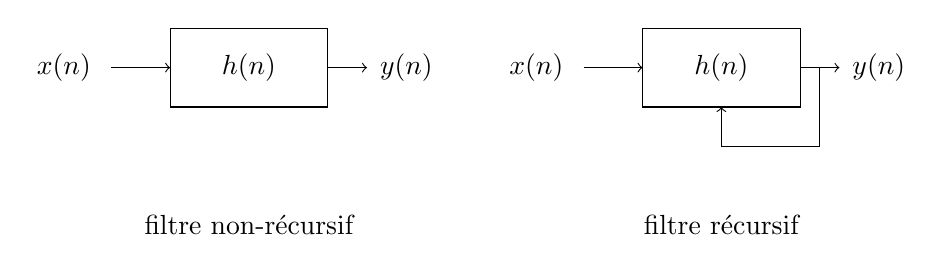
\begin{tikzpicture}
	%\draw (2.15,-1.5) node {Glc};
	%\draw[->] (2.15,-1)-- (2.15,-0.5);
	%\draw (1.25,-0.5) rectangle(3,0.5);
	\draw (2.15,0) node {$x(n)$};
	%\draw[->] (2.15,0.5)-- (2.15,1);
	%\draw (2.15,1.5) node {ATP};
	
	\draw[->] (2.75,0)-- (3.5,0);
	\draw (3.5,-0.5) rectangle(5.5,0.5) ;
	\draw (4.5,0) node {$h(n)$};
	%\draw[->] (4.5,0.5) arc(90:60:0.5);
	%\draw[->] (4.5,-0.5) arc(-90:-120:0.5);
	%\draw[->] (4.5,-1)-- (4.5,-0.5);
	%\draw (4.5,-1.5) node {Glt};
	%\draw[->] (4.5,0.5)-- (4.5,1);
	%\draw (4.5,1.5) node {ATP};
	
	\draw[->] (5.5,0)-- (6,0);
	%\draw[->] (6,-0.5) rectangle(7,0.5); 
	\draw (6.5,0) node {$y(n)$};
	%\draw[->] (6.5,-1)-- (6.5,-0.5);
	%\draw (6.5,-1.5) node {O$_2$};
	%\draw[->] (6.5,0.5)-- (6.5,1);
	%\draw (6.5,1.5) node {ATP};
	\draw (4.5,-2) node {filtre non-récursif};
	
	
		%\draw (2.15,-1.5) node {Glc};
	%\draw[->] (2.15,-1)-- (2.15,-0.5);
	%\draw (1.25,-0.5) rectangle(3,0.5);
	\draw (8.15,0) node {$x(n)$};
	%\draw[->] (2.15,0.5)-- (2.15,1);
	%\draw (2.15,1.5) node {ATP};
	
	\draw[->] (8.75,0)-- (9.5,0);
	\draw (9.5,-0.5) rectangle(11.5,0.5) ;
	\draw (10.5,0) node {$h(n)$};
	%\draw[->] (4.5,0.5) arc(90:60:0.5);
	%\draw[->] (4.5,-0.5) arc(-90:-120:0.5);
	%\draw[->] (4.5,-1)-- (4.5,-0.5);
	%\draw (4.5,-1.5) node {Glt};
	%\draw[->] (4.5,0.5)-- (4.5,1);
	%\draw (4.5,1.5) node {ATP};
	
	\draw[->] (11.5,0)-- (12,0);
	%\draw[->] (6,-0.5) rectangle(7,0.5); 
	\draw (12.5,0) node {$y(n)$};
	%\draw[->] (6.5,-1)-- (6.5,-0.5);
	%\draw (6.5,-1.5) node {O$_2$};
	%\draw[->] (6.5,0.5)-- (6.5,1);
	%\draw (6.5,1.5) node {ATP};
	\draw (10.5,-2) node {filtre récursif};
	
	\draw[-] (11.75,0)-- (11.75,-1);
	\draw[-] (11.75,-1)-- (10.5,-1);
	\draw[->] (10.5,-1)-- (10.5,-0.5);
	\end{tikzpicture}
\end{center}

Un exemple très simple de filtre non-récursif est le filtre défini par la relation :

\[ y(n) = \frac{x(n) + x(n-1)}{2}  \]\\

De la même manière une filtre récursif très simple peut être défini de la manière suivante.\\

\[ y(n) = \frac{x(n) + y(n-1)}{2}  \]\\

Cette catégorisation va rester importante tout au long de ce cours car ces deux familles de filtres ont des propriétés assez différentes, notamment en terme de stabilité.\\

Cette façon d'écrire la sortie du filtre à l'échantillon $n$ en fonction des échantillons de sortie et d'entrée à d'autres instants s'appelle \textbf{l'équation de récurrence du filtre} et c'est une des trois manières de définir un filtre linéaire invariant dans le temps.  

\subsection{Notion de fonction de transfert et réponse impulsionnelle} 

\textbf{Question: Que vous évoque la notion de fonction de transfert ?}\\

Pour les systèmes continus invariant linéaires dans le temps, la fonction de transfert est définie comme le rapport de la transformée de Laplace du signal de sortie et du signal d'entrée : $H(s) = \frac{Y(s)}{X(s)}$. Dans le cas d'un système discret on définit la fonction de transfert comme le rapport de la transformée en Z de la suite de sortie et de la suite d'entrée: $H(z) = \frac{Y(z)}{X(z)}$\\

Il s'avère par ailleurs que la fonction de transfert du filtre est tout simplement la transformée de Fourier de sa réponse impulsionnelle. En effet, les systèmes discrets linéaires invariants dans le temps sont définis comme suit:\\

\[ y(n) = \sum_{m = 0}^{N-1} h(m) x(n-m) =  h(n)\star x(n) \]\\ 

Si on prend la transformée en Z de cette relation on obtient l'équation suivante :

\[ Y(z) = TZ(h(n)\star x(n)) =  H(z) X(z) \rightarrow  H(z) = \frac{Y(z)}{X(z)}\]\\ 

\textbf{Exercice: Calculer la fonction de transfert des filtres caractérisés par les équations de récurrence suivantes :}\\
\begin{enumerate}
\item  $y_1(n) = \frac{x_1(n) + x_1(n-1)}{2}$
\item  $y_2(n) = \frac{x_2(n) + y_2(n-1)}{2}$
\end{enumerate}


\textbf{1. $y_1(n) = \frac{x_1(n) + x_1(n-1)}{2}$}


On sait déjà que la fonction de transfert s'établit, non pas sur les suites, mais sur la transformée en Z dans le cas des signaux discrets. On commence donc par appliqué la transformée en Z à l'équation de récurrence:\\

\[ y_1(n) = \frac{x_1(n) + x_1(n-1)}{2} \rightarrow Y_1(z) = \frac{X_1(z) + X_1(z)z^{-1}}{2} \]

\[ Y_1(z) = \frac{X_1(z) + X_1(z)z^{-1}}{2} \rightarrow Y_1(z) = X_1(z)\frac{(1 + z^{-1})}{2}  \]

\[  \rightarrow \frac{Y_1(z)}{X_1(z)} = H_1(z) = \frac{(1 + z^{-1})}{2}  \]\\

\textbf{2. $y_2(n) = \frac{x_2(n) + y_2(n-1)}{2}$}


On sait déjà que la fonction de transfert s'établit, non pas sur les suites, mais sur la transformée en Z dans le cas des signaux discrets. On commence donc par appliqué la transformée en Z à l'équation de récurrence:\\

\[ y_2(n) = \frac{x_2(n) + y_2(n-1)}{2} \rightarrow Y_2(z) = \frac{X_2(z) + Y_2(z)z^{-1}}{2} \]

\[ Y_2(z) = \frac{X_2(z) + Y_2(z)z^{-1}}{2} \rightarrow Y_2(z)(1-\frac{z^{-1}}{2}) = \frac{X_2(z)}{2}  \]

\[  \rightarrow \frac{Y_2(z)}{X_2(z)} = H_2(z) = \frac{1}{2}\frac{1}{(1 - \frac{z^{-1}}{2})}  \]\\


Arrêtons nous quelques instants pour discuter de la forme des fonctions de transferts de ces deux filtres. Dans le cas du filtre non-récursif, on constate que les termes en $z$ (qui traduisent l'intervention d'échantillons plus ou moins retardés dans la réponse du système) sont tous au numérateur. alors que dans le cas du filtre récursif récursive, il y en a également au dénominateur. On note alors que dans le cas du filtre récursif, si $z{-1}$ prend un valeur qui annule le dénominateur la fonction de transfert diverge. C'est une des signes d'instabilité. 

\textbf{Exercice: Calculer la réponse impulsionnelle des filtres au fonction de transferts suivantes :}
\begin{enumerate}
\item  $H_1(z) = \frac{(1 + z^{-1})}{2}$
\item  $H_2(z) = \frac{1}{2}\frac{1}{(1 - \frac{z^{-1}}{2})}$
\end{enumerate}

\textbf{1. $H_1(z) = \frac{(1 + z^{-1})}{2}$}\\

La transformée en Z étant linéaire, on peut traiter chaque terme de la somme séparément.\\

On sait que la fonction dont la transformée en Z est la fonction unité est l'impulsion de Kronecker $\delta(n)$. Le premier terme correspond donc à $\frac{\delta(n)}{2}$.\\

On sait également que la transformée d'un signal retardé de k échantillon revient à multiplier $ z^{-k}$. Ce terme en $ z^{-k}$ correspond donc à une terme dont la transformée en Z est la fonction unité retardé d'un échantillon, c'est-à-dire $\frac{\delta(n-1)}{2}$.\\

Donc au final on obtient : 

\[h_1(n) = \frac{\delta(n)}{2} - \frac{\delta(n-1)}{2}\]\\

Dans ce cas précis, il est intéressant de faire le même exercice en partant cette fois de l'équation de récurrence. Pour ce faire on reprend l'équation de récurrence en remplaçant $x(n)$, le signal d'entrée par une impulsion de Kronecker. On obtient alors exactement la même expression que précédemment.\\ 

\begin{center}
\begin{tikzpicture}

	\draw[->] (-3,0)-- (3,0);
\draw (-0,-0.3) node {0};
\draw[->] (0,0)-- (0,1.5);
\draw (3.1,0.25) node {$n$};
\draw (0,2) node {$h_1(n)$};
%\draw (4.5,-0.3) node {1};



\draw[->,blue,thick](-3,0)--(-3,0);
\draw[->,blue,thick](-2,0)--(-2,0);
\draw[->,blue,thick](-1,0)--(-1,0);
\draw[->,blue,thick](0,0)--(0,0.5);
\draw[->,blue,thick](1,0)--(1,0.5);
\draw[->,blue,thick](2,0)--(2,0);
\draw[->,blue,thick](3,0)--(3,0);


\end{tikzpicture}
\end{center}


\textbf{2. $H_2(z) = \frac{1}{2}\frac{1}{(1 - \frac{z^{-1}}{2})}$}\\

Dans ce cas, si on reprend le tableau des transformées usuelles on constate que $H_2(z)$ est à un facteur près, précisément la transformée en Z de la fonction échelon unité $u(n)$. Donc, 

\[h_2(n) = \frac{-0.5^n u(n)}{2}\]\\

Dans ce cas calculer cette réponse directement à partir de l'équation de récurrence est moins direct que dans le cas du filtre non-récursif. En effet si on remplace $x(n)$, le signal d'entrée par une impulsion de Kronecker dans l'équation de récurrence, on obtient :

\[h_2(n) = \frac{\delta(n) + h_2(n-1)}{2}\]\\

Pour pouvoir poursuivre il faut calculer $h_2(n)$ sur quelques échantillons. Pour $n$ négatif, on sait que l'entrée est nulle et l'échantillon précédent également. Pour $n=0$, l'entrée prend la valeur 1 mais l'échantillon précédent vaut toujours zéro donc la sortie vaut vaut 1/2 au temps zéro. Pour l'échantillon 1, l'entrée revient à la valeur nulle mais la sortie précédente vaut 1/2 et la facteur$ \frac{1}{2}$ donne $h_2(1) = \frac{1}{4}$. à l'échantillon suivant la valeur précédente est à nouveau divisée par deux et ainsi de suite.

\begin{center}
\begin{tikzpicture}

	\draw[->] (-3,0)-- (3,0);
\draw (-0,-0.3) node {0};
\draw[->] (0,0)-- (0,1.5);
\draw (3.1,0.25) node {$n$};
\draw (0,2) node {$h_1(n)$};
%\draw (4.5,-0.3) node {1};



\draw[->,blue,thick](-3,0)--(-3,0);
\draw[->,blue,thick](-2,0)--(-2,0);
\draw[->,blue,thick](-1,0)--(-1,0);
\draw[->,blue,thick](0,0)--(0,1);
\draw[->,blue,thick](1,0)--(1,0.5);
\draw[->,blue,thick](2,0)--(2,0.25);
\draw[->,blue,thick](3,0)--(3,0.125);


\end{tikzpicture}
\end{center}

\subsubsection{Réponse impulsionnelle finie et infinie}
Dans les deux exercices précédents, on a traité un filtre non-récursif et un filtre non-récursif. On a pu constater que dans le cadre du filtre non-récursif, la réponse impulsionnelle présentait un nombre fini d'échantillons non nul. \`A l'inverse le filtre récursif, du fait de la contribution de l'échantillon précédente à une réponse impulsionnelle comportant un nombre infini d'échantillons non nul.\\

Cette observation peut se généraliser à l'ensemble des filtres récursifs et non-récursifs. On dit alors que les filtres récursifs sont des \textbf{filtres à réponse impulsionnelles infinie} (RII) et les filtres non-récursifs sont des \textbf{filtres à réponse impulsionnelle finie} (RIF). Dans les sous-sections suivantes nous allons aborder les implications de cette distinction.

\section{Filtres à réponse impulsionnelle finie}
Un filtre à réponse impulsionnelle finie ou récursif est un filtre qui ne fait appel pour le calcul de la sortie qu'au coefficient de l'entrée. On dit qu'il ne comporte pas de \textbf{rétroaction}. Soit $x[n]$ et $y[n]$  respectivement les signaux d'entrée et de sortie d'un filtre à réponse impulsionnelle finie, on peut écrire la relation suivante : 

\[ y[n] =  \sum_{k = 0}^{N-1} a_k \; x[n-k]\] 

où $N$ est le nombre de coefficient et les $a_k$ sont les coefficients de la fonction de transferts. Maintenant, si on écrit la transformée en Z de cette équation, on obtient :

\[ Y(z) =  \sum_{k = 0}^{N-1} a_k \; X(z)z^{-k} \] 

On va d'abord étudier deux exemples simples de filtres à réponse impulsionnelle finie et analyser leur caractéristiques pour en tirer des concepts généraux sur ce type de filtre.

\subsection{Exemple de filtres à réponse impulsionnelle finie}
Le premier exemple est le filtre suivant : 

\[ y(nT_e) = \frac{1}{2}[x(nT_e) + x((n-1)T_e)  ] \]\\

\textbf{Questions : Quel est l'outil mathématique utilisée ici pour définir le filtre ? Quels sont les autres définitions possibles pour un filtre linéaire invariant dans le temps ?  }\\

L'équation de récurrence du filtre a été donné mais on aurait également pu donner sa fonction de transfert ou sa réponse impulsionnelle afin de décrire sa réponse.\\

\textbf{Exercice : Calculer la fonction de transfert du filtre précédent. }\\

Pour calculer la fonction de transfert on calcule la transformée en Z de l'équation de récurrence 

\[ Y(z) = \frac{1}{2}[X(z) + X(z)z^{-1}  ] \]
\[ Y(z) = X(z)\frac{1}{2}[1 + z^{-1}  ] \]
\[ H(z) = \frac{Y(z)}{X(z)} = \frac{1}{2}[1 + z^{-1}  ] \]\\

Ici, pour aller plus loin dans l'analyse du système, on passe de la transformée en z à la transformée de Fourier  en effectuant un changement de variable $z = e^{j\pi f T_e}$. \\

\[ H(z) = \frac{Y(z)}{X(z)} = \frac{1}{2}[1 + z^{-1}  ] \rightarrow H(f) = \frac{1}{2}[1 + e^{j2\pi f T_e}]\]\\

\textbf{Exercice : Calculer le spectre}\\

Le spectre du signal est, on le  rappelle, le couple module et argument de la fonction complexe que représente la transformée de  Fourier. à ce stade il est important de réaliser que bien que la fonction soit discrète la transformée de Fourier est ici bien une fonction continue.\\

On commence par calculer le module :\\

\[ |H(f)| = |\frac{1}{2}[1 + e^{-j2\pi f T_e}]| = |\frac{1}{2}e^{-j\pi f T_e}[e^{j\pi f T_e} + e^{-j\pi f T_e}]|   \]

\[ |H(f)| = |e^{-j\pi f T_e}\cos(\pi f T_e)|  = |\cos(\pi f T_e)|   \]

à partir de l'expression précédente on peut également extraire le module facilement : 

\[ arg(H(f)) = arg(e^{-j\pi f T_e}\cos(\pi f T_e)) = \pi f T_e\]

On constate que la phase du filtre dépend linéairement de la fréquence pour  ce type de filtre.

\begin{center}
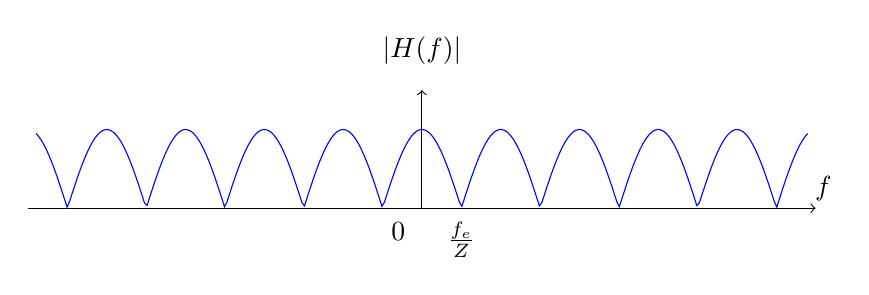
\begin{tikzpicture}

	\draw[->] (-5,0)-- (5,0);
\draw (-0.3,-0.3) node {0};
\draw[->] (0,0)-- (0,1.5);
\draw (5.1,0.25) node {$f$};
\draw (0,2) node {$|H(f)|$};
\draw (0.5,-0.4) node {$\frac{f_e}{Z}$};

\draw[domain=-4.9:4.9,color=blue,samples=300] plot (\x,{abs(cos(3.14 *\x r))});
\end{tikzpicture}
\end{center}

On constate que ce filtre coupe complètement les composantes du signal dont la fréquence est égale au double de la fréquence d'échantillonnage. Cela provient de l'effet de moyennage sur deux échantillons.

On note que la phase du filtre évolue linéairement avec la fréquence d'excitation. Ceci va nous permettre d'introduire la notion de filtre à phase linéaire.

\subsection{Notion de phase linéaire et filtrage à déphasage linéaire}
Un filtre est dit à phase linéaire si sa fonction de transfert peut s'écrire de la façon suivante: 

\[ H(f) = R(f)e^{-j(2\pi f \tau +\phi_0)} \]

Le fait que la phase soit une fonction affine de la fréquence a des conséquences importantes pour le traitement du signal qu'on va illustrer par un exemple :

\begin{center}
\begin{tikzpicture}

	\draw[->] (-3,0)-- (3,0);
\draw (-0.3,-0.3) node {0};
\draw[->] (0,-1.5)-- (0,1.5);
\draw (3.1,0.25) node {$f$};
\draw (0,2) node {$g(t)$};
%\draw (0.5,-0.4) node {$\frac{2}{T_e}$};

\draw[domain=-2.9:2.9,color=blue,samples=300] plot (\x,{0.5*cos(2*\x r) + 0.5*cos(4*\x r)});
\end{tikzpicture}
\end{center}

On a tracé ici la fonction suivante : 

\[ g(t) = \frac{1}{2} \cos(2 x) + \cos(4 x) \]\\

Appliquons maintenant un déphasage de $\pi/6$ aux  deux composantes fréquentielles que contient ce signal : $\frac{1}{pi}$  et $\frac{2}{pi}$. La fonction devient alors : \\

\[ g_1(t) = \frac{1}{2} \cos(2 x + \pi/6) + \cos(4 x +  \pi/6) \]\\

Si on trace $g_1(t)$, on fait le constat suivant.

\begin{center}
\begin{tikzpicture}

	\draw[->] (-3,0)-- (3,0);
\draw (-0.3,-0.3) node {0};
\draw[->] (0,-1.5)-- (0,1.5);
\draw (3.1,0.25) node {$f$};
\draw (0,2) node {$g_1(t)$};
%\draw (0.5,-0.4) node {$\frac{2}{T_e}$};

\draw[dotted, domain=-2.9:2.9,color=blue,samples=300] plot (\x,{0.5*cos(2*\x r  ) + 0.5*cos(4*\x r )});

\draw[domain=-2.9:2.9,color=blue,samples=300] plot (\x,{0.5*cos(2*\x r +3.14/6 r ) + 0.5*cos(4*\x r + 3.14/6 r)});
\end{tikzpicture}
\end{center}

Si on compare le signal avec ces deux composantes déphasées de la même valeur au signal original on se rend compte que le signal n'a pas simplement été décalé vers la droite ou vers la gauche, mais qu'il a également subit une légère distorsion.\\

Prenons un le signal $g_2(t)$ suivant: 
\[ g_2(t) = \frac{1}{2} \cos(2 x + \pi/6 + \pi/6*\frac{1}{\pi}) + \cos(4 x +  \pi/6 + \pi/6*\frac{2}{\pi})  \]

Cette fois-ci, on a introduit un déphasage proportionnel à la fréquence de chaque composante. Cette fois ci, on constate en traçant la fonction que ce déphasage linéaire induit un décalage sans distorsion du signal.

\begin{center}
\begin{tikzpicture}

	\draw[->] (-3,0)-- (3,0);
\draw (-0.3,-0.3) node {0};
\draw[->] (0,-1.5)-- (0,1.5);
\draw (3.1,0.25) node {$t$};
\draw (0,2) node {$g_1(t)$};
%\draw (0.5,-0.4) node {$\frac{2}{T_e}$};

\draw[dotted, domain=-2.9:2.9,color=blue,samples=300] plot (\x,{0.5*cos(2*\x r  ) + 0.5*cos(4*\x r )});

\draw[domain=-2.9:2.9,color=blue,samples=300] plot (\x,{0.5*cos(2*\x r +2/6 r) + 0.5*cos(4*\x r  + 4/6 r)});
\end{tikzpicture}
\end{center}

Donc en traitement du signal, avoir une phase linéaire en fréquence permet de transporter le signal à travers le filtre \textbf{sans distorsion.}\\

Maintenant que les implications de la linéarité de la phase ont été rappelé, on peut se poser la question de ses implications notamment dans le cadre de l'étude des filtres à réponse impulsionnelle finie (RIF).\\

La principale implication de la linéarité de la phase dans le filtrage est que si le signal met un temps $\tau$ à se propager à travers le filtre, alors, la réponse impulsionnelle du filtre, c'est-à-dire dans le domaine \textit{temporel} doit être \textbf{symétrique par rapport à $\tau$}. Le détail précis de cette démonstration est technique sur le plan mathématique et n'apporte que peu à la compréhension globale de la notion on va donc se concentrer dans la suite sur la synthèse de filtres RIF.\\ 

Les filtres à réponse impulsionnelle ont deux avantages principaux: Ils sont inconditionnellement stables et permettent le filtrage à phase linéaire. Pour la stabilité on résumera simplement en disant qu'une entrée bornée (au sens de son amplitude) résulte forcément en une sortie bornée, mais cette notion sera abordée plus en détail dans la partie sur les filtres à réponse impulsionnelle infinie.\\

\subsection{Synthèse de filtres non récursif/filtres à réponse impulsionnelle finie} 
Avant toute chose on va discuter la notion même de synthèse de filtre.\\

\textbf{Question: Que vous évoque la notion de synthèse de filtre ?}\\

Comme dans beaucoup de problèmes d'ingénierie, la synthèse de filtre va consister à atteindre un objectif chiffré avec une certaine tolérance autour de cette objectif. Dans le cadre des filtres, il s'agit d'obtenir un filtre avec des caractéristiques dans une certaine tolérance.\\

On rappelle qu'un filtre, s'il est linéaire invariant dans le temps, est caractérisé de façon équivalente par sa fonction de transfert (domaine de Fourier/Laplace/Z), sa réponse impulsionnelle, ou bien une équation (domaine temporel), différentielle pour les filtres continues ou de récurrence pour les filtres numériques.\\

En général pour définir le filtre qu'on souhaite synthétiser on part du domaine fréquentielle. C'est donc la fonction de transfert (sa partie réelle ET sa partie imaginaire) qu'on va chercher à définir et sur lesquelles on va appliquer des contraintes et des tolérances.\\

Le point de départ est donc généralement ce qu'on va appeler un \textbf{gabarit} qui va définir les contraintes et tolérances sur le module de la fonction de transfert $H(f)$ à déterminer.

\begin{center}
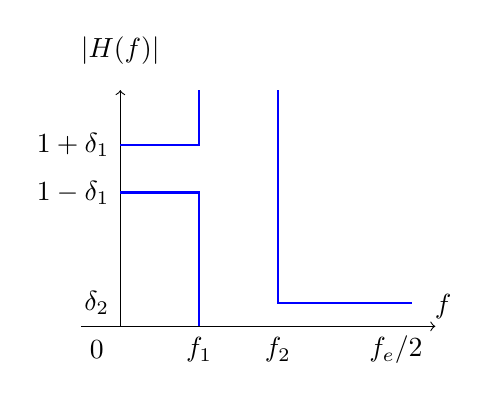
\begin{tikzpicture}

	\draw[->] (-0.5,0)-- (4,0);
\draw (-0.3,-0.3) node {0};
\draw[->] (0,0)-- (0,3);
\draw (4.1,0.25) node {$f$};
\draw (0,3.5) node {$|H(f)|$};
\draw (1,-0.3) node {$f_1$};
\draw (2,-0.3) node {$f_2$};
\draw (-0.6,1.7) node {$1 - \delta_1$};
\draw (-0.6,2.3) node {$1 + \delta_1$};
\draw (-0.3,0.3) node {$\delta_2$};
\draw (3.5,-0.3) node {$f_e/2$};


\draw[thick,blue](0,1.7)--(1,1.7)--(1,0);
\draw[thick,blue](0,2.3)--(1,2.3)--(1,3);
\draw[thick,blue](2,3)--(2,0.3)--(3.7,0.3);

\end{tikzpicture}
\end{center}

\textbf{Question: Pourquoi ce gabarit s'arrête-t-il à $f_e/2$ ?}

Ici, si on considère qu'on travaille avec un filtre numérique avec une fréquence d'échantillonnage $f_e$, alors on sait que le spectre du signal échantillonné correspond au spectre du signal continu dupliqué dans son intégralité à chaque $f_e$ dans le domaine fréquentiel. En d'autres termes le fonction $|H(f)|$ est périodique de période $f_e$ et donc il est inutile de représenter plus que l'intervalle [$-f_e/2;f_e/2$].\\

Dans les faits, pour les filtres numériques, on règle généralement les échantillons $h_i$ du filtre dans le domaine \textbf{temporel} afin que la fonction périodique $|H(f)|$ ait les caractéristiques correspondant au gabarit. Une fois le gabarit établi, il existe plusieurs méthodes pour calculer une réponse impulsionnelle remplissant ses conditions, dont :
\begin{itemize}
\item Développement en série de Fourier
\item Méthode des moindres carrés
\item Méthode par Transformée de Fourier Discrète (TFD)
\item Méthode par approximation de Tchebychev
\end{itemize}

On va à minima présenter ces méthodes, mais avant on va fixer les idées en travaillant sur un premier exemple: le filtre passe-bas idéal. Le but étant ici de fixer les idées et concepts qui seront remis en oeuvre pour des synthèse de filtres plus complexes.\\

\subsubsection{Étude du filtre passe-bas idéal}

\begin{center}
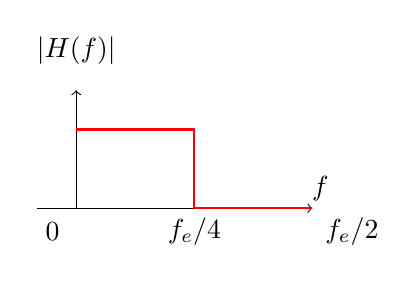
\begin{tikzpicture}

	\draw[->] (-0.5,0)-- (3,0);
\draw (-0.3,-0.3) node {0};
\draw[->] (0,0)-- (0,1.5);
\draw (3.1,0.25) node {$f$};
\draw (0,2) node {$|H(f)|$};
\draw (1.5,-0.3) node {$f_e/4$};
\draw (3.5,-0.3) node {$f_e/2$};


\draw[thick,red](0,1)--(1.5,1)--(1.5,0)--(3,0);


\end{tikzpicture}
\end{center}

Le filtre numérique représenté juste au-dessus coupe intégralement toutes les fréquences supérieure à $f_e/4$. Maintenant on peut connaître la forme de la réponse impulsionnelle échantillonnée à partir de cette fonction de transfert.\\

Puisque la fonction de transfert est périodique de période $f_e$, elle correspond forcément à un signal échantillonné. il faut maintenant savoir quel est ce signal. Et en l'occurrence on sait, que la transformée de  Fourier du signal rectangulaire est la fonction sinus cardinal. Donc en connaissant les propriétés de la transformée de Fourier et les transformées usuelles on peut en déduire les échantillons de la forme de la réponse impulsionnelle.\\

\begin{center}
\begin{tikzpicture}

	\draw[->] (-0.5,0)-- (3,0);
\draw (-0.3,-0.3) node {0};
\draw[->] (0,0)-- (0,1.5);
\draw (3.1,0.25) node {$f$};
\draw (0,2) node {$|H(f)|$};
\draw (1.5,-0.3) node {$f_e/4$};
\draw (3.5,-0.3) node {$f_e/2$};


\draw[thick,red](0,1)--(1.5,1)--(1.5,0)--(3,0);

\draw[->] (3.5,1)-- (4.5,1);

\draw[->] (7.5,0)-- (7.5,1.5);
\draw (7.5,-0.3) node {0};
\draw[->] (5,0)-- (10,0);
\draw (10.1,0.25) node {$t$};
\draw (7.5,2) node {$h(t)$};
\draw[dotted, domain=4.9:9.9,color=red,samples=80] plot (\x,{80*sin(5*3.14*\x r -5*3.14*7.5r )/(5*3.14*\x r-5*3.14*7.5 r)});

\draw[red] (7.5,0)-- (7.5,1.4);
\draw[red] (7.75,0)-- (7.75,-0.25);
\draw[red] (7.25,0)-- (7.25,-0.25);
\draw[red] (8,0)-- (8,0.17);
\draw[red] (7,0)-- (7,0.17);
\draw[red] (8.25,0)-- (8.25,-0.1);
\draw[red] (6.75,0)-- (6.75,-0.1);
\draw[red] (8.5,0)-- (8.5,0.01);
\draw[red] (6.5,0)-- (6.5,0.01);
\draw[red] (8.75,0)-- (8.75,0.07);
\draw[red] (6.25,0)-- (6.25,0.07);
\draw[red] (9,0)-- (9,-0.075);
\draw[red] (6,0)-- (6,-0.075);
\draw[red] (9.25,0)-- (9.25,0.03);
\draw[red] (5.75,0)-- (5.75,0.03);
\draw[red] (9.5,0)-- (9.5,-0.01);
\draw[red] (5.5,0)-- (5.5,-0.01);
\draw[red] (9.75,0)-- (9.75,-0.02);
\draw[red] (5.25,0)-- (5.25,-0.02);
\end{tikzpicture}
\end{center}

La réponse impulsionnelle de ce filtre correspond donc à l'échantillonnage de la fonction \textbf{sinus cardinal}. Cependant, cette réponse impulsionnelle ne correspond pas à un filtre à réponse impulsionnelle finie. Elle peut s'en approcher mais ne l'est pas rigoureusement.\\

Afin de rendre la réponse impulsionnelle finie, on peut fenêtrer la fonction $h(t)$ dans le domaine temporel. Cela veut dire qu'on va la multiplier par une fonction rectangulaire de la largeur souhaitée. Cela signifie quand dans le domaine de Fourier, la fonction de transfert va être convoluée à la transformée de Fourier de la fonction fenêtre choisie.\\

\begin{center}
\begin{tikzpicture}

\draw[->] (7.5-7,0)-- (7.5-7,1.5);
\draw (7.5-7,-0.3) node {0};
\draw[->] (5-7,0)-- (10-7,0);
\draw (10.1-7,0.25) node {$t$};
\draw (7.5-7,2) node {$h(t)$};
\draw[dotted, domain=4.9-7:9.9-7,color=red,samples=80] plot (\x,{80*sin(5*3.14*\x r -5/2*3.14 r )/(5*3.14*\x r - 5/2*3.14 r)});

\draw[red] (7.5-7,0)-- (7.5-7,1.2);
\draw[red] (7.75-7,0)-- (7.75-7,-0.25);
\draw[red] (7.25-7,0)-- (7.25-7,-0.25);
\draw[red] (8-7,0)-- (8-7,0.17);
\draw[red] (7-7,0)-- (7-7,0.17);
\draw[red] (8.25-7,0)-- (8.25-7,-0.1);
\draw[red] (6.75-7,0)-- (6.75-7,-0.1);
\draw[red] (8.5-7,0)-- (8.5-7,0.01);
\draw[red] (6.5-7,0)-- (6.5-7,0.01);
\draw[red] (8.75-7,0)-- (8.75-7,0.07);
\draw[red] (6.25-7,0)-- (6.25-7,0.07);
\draw[red] (9-7,0)-- (9-7,-0.075);
\draw[red] (6-7,0)-- (6-7,-0.075);
\draw[red] (9.25-7,0)-- (9.25-7,0.03);
\draw[red] (5.75-7,0)-- (5.75-7,0.03);
\draw[red] (9.5-7,0)-- (9.5-7,-0.01);
\draw[red] (5.5-7,0)-- (5.5-7,-0.01);
\draw[red] (9.75-7,0)-- (9.75-7,-0.02);
\draw[red] (5.25-7,0)-- (5.25-7,-0.02);

\draw[->] (10.5-7,1)-- (11.5-7,1);
\draw(11-7,0.5) node {fenêtre};

\draw[->] (7.5,0)-- (7.5,1.5);
\draw (7.5,-0.3) node {0};
\draw[->] (5,0)-- (10,0);
\draw (10.1,0.25) node {$t$};
\draw (7.5,2) node {$h(t)$};
\draw[dotted, domain=6.75:8.25,color=red,samples=80] plot (\x,{80*sin(5*3.14*\x r -5*3.14*7.5 r )/(5*3.14*\x  r-5*3.14*7.5 r)});

\draw[red] (7.5,0)-- (7.5,1.3);
\draw[red] (7.75,0)-- (7.75,-0.25);
\draw[red] (7.25,0)-- (7.25,-0.25);
\draw[red] (8,0)-- (8,0.17);
\draw[red] (7,0)-- (7,0.17);
\draw[red] (8.25,0)-- (8.25,-0.1);
\draw[red] (6.75,0)-- (6.75,-0.1);
\draw[blue,dashed,thick] (5,0)--(6.75,0)--(6.75,1.7)--(8.25,1.7)--(8.25,0)--(10,0);


\end{tikzpicture}
\end{center}

Dans la figure précédente, on a rendu la réponse impulsionnelle finie dans le temps en utilisant une fenêtre rectangulaire. Si on se rappelle de la relation entre multiplication et convolution sur les espaces dual que sont les espaces de Fourier et l'espace direct, on sait que multiplier la réponse impulsionnelle par une fonction rectangulaire revient à convoluer la transformée de Fourier de la réponse impulsionnelle par la transformée de Fourier de la fenêtre.\\

\[ H(f) =  \int^{\infty}_{-\infty} \frac{\sin(\phi)}{\phi } \Pi_L(f- \phi) d \phi \]
\[ H(f) =  \int^{L/2+f}_{-(L/2+ f)} \frac{\sin(\phi)}{\phi }  d \phi \]

Cette quantité peut se calculer assez facilement sous MATLAB. la forme de cette fonctioin a été tracée dans la figure suivante:\\ %integral(@sinc,-8,12)


\usetikzlibrary {datavisualization}
\input{convoplot}
%
%\begin{center}
%\begin{tikzpicture}
%  \datavisualization [scientific axes, x axis={length=4 cm}, visualize as smooth line = hf, hf ={style = blue}]
%	data [read from file=HF.csv];
%\end{tikzpicture}
%\end{center}

%\usetikzlibrary {datavisualization.formats.functions}
%\begin{tikzpicture}
%  \datavisualization [scientific axes,x axis={length=3cm, ticks=few}, visualize as smooth line]
%    data [format=function] {var x : interval [-1.5:1.5] samples 7;
%      func y = \value x*\value x; };
%\end{tikzpicture}

Par ailleurs, cette propriété est très bien illustrée par le fait que si on cherche à tracer la fft de la fonction sinus cardinal dans MATLAB, on obtient pas la fonction rectangulaire, mais une fonction approchée comportant des oscillations.\\

Ici, la fenêtre temporelle qui rend la réponse impulsionnelle finie a été prise rectangulaire et cela a eu un impact sur la fonction de transfert du spectre en y ajoutant des oscillations d'une certaine amplitude et avec une certaine période dans le spectre. Si une fonction différente était choisie, ces oscillations aurait des caractéristiques différentes. C'est le principe de la \textbf{méthode des fenêtres.}\\

Ce qu'il faut comprendre avant d'aller plus loin, c'est que si la fonction correspondant parfaitement à un gabarit existe \textit{mathématiquement}, elle ne peut pas correspondre à un filtre réel, c'est-à-dire avec un nombre fini d'échantillons dans sa réponse impulsionnelle. Les oscillations dans la fonction de transfert du filtre réel sont la conséquence du nombre fini d'échantillons.\\

\subsubsection{Méthodes basées sur la réponse impulsionnelle}
On peut procéder de plusieurs façon pour passer du gabarit d'un filtre à se réponse en fréquence "concrète". On va surtout se concentrer ici sur les principes généraux inhérents à la synthèse de filtres numériques non-récursifs.

\begin{enumerate}
\item On fixe une contrainte sur la suite  représentant spectre échantillonné $H_k$ ou sur $H(f)$ 
\item On en déduit une la suite  $h_i$ correspondant à la réponse impulsionnelle du filtre numérique correspondant
\item Cette suite $h_i$ déduite directement ne respecte généralement pas toutes les contraintes souhaitées 
\item On change alors le nombre d'échantillons  et/ou on pondère la réponse impulsionnelle pour obtenir une suite ayant une transformée de Fourier $H*(f)$ qui aura les bonnes caractéristiques.
\end{enumerate}

Toutes les méthodes suivent ce principe général. Il faut donc comprendre qu'elles reposent gloabelement toutes sur l'enchaînement suivant détaillé dans le schéma suivant :

\begin{center}
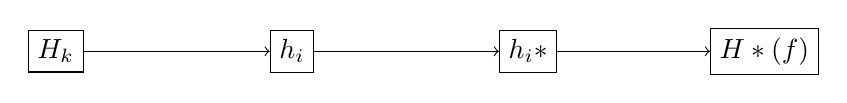
\begin{tikzpicture}
		\node[rectangle,draw,align=center] (I) at (1,0) {$H_k$};
		\node[rectangle,draw,align=center] (D) at (4,0) {$h_i$};
		\node[rectangle,draw,align=center] (N) at (7,0) {$h_i*$};
		\node[rectangle,draw,align=center] (B) at (10,0) {$H*(f)$};	
		
		\draw[->] (I)--(D);
		\draw[->] (D)--(N);
		\draw[->] (N)--(B);
\end{tikzpicture}
\end{center}
On passe donc des échantillons  prédeterminés $H_k$ à la réponse impulsionnelle "préliminaire" $h_i$ qui ne correspondra pas aux contraintes, qu'on modifie en $h_i*$ afin de satisfaire les dites contraintes, et qui aura elle une transformée de Fourier $H*(f)$ avec les bonnes propriétés.\\

Maintenant qu'on a présenté le principe général, on va pouvoir détailler quelques unes de ces méthodes et expliquer leur propriétés.

\paragraph{Méthodes des fenêtres} 
La méthode des fenêtres est la plus "directe", et historiquement la première. C'est généralement avec cette dernière  qu'on présente le principe de la synthèse de filtre. Avec cette méthode, une fois la suite des $h_i$ obtenues, on applique une fenêtre pour obtenir une suite des $h_i*$ correspondant à une gabarit.\\

\textbf{[schéma]}\\

En revanche, une caractéristique des filtres numériques synthétisés par le biais de cette méthode est que l'amplitude des oscillations en bande passante et affaiblie est reliée à la largeur de la bande de transition. Ainsi si on souhaite avoir une amplitude faible en bande de transition, on aura nécessairement une bande de transition large. On notera également que les oscillations d'amplitude non constante et similaire en bande passante et affaiblie.\\

De façon plus général, il faut comprendre que la fenêtre "fixe" des caractéristiques tels que les fréquences de transition de la bande passante et de la bande affaiblie et qu'il n'y a pas de méthode simple pour faire évoluer un seul de ces paramètres en conservant les autres.

\paragraph{Méthode de l'échantillonnage en fréquence}
Cette méthode consiste à passer par des calculs dans le domaine fréquentiel pour obtenir les $h_i$ correspondant à une fonction $H(f)$ satisfaisant les critères souhaités.\\

Le principe général de la méthode consiste à fixer/choisir des échantillons sur spectre $H_k$ avec les bonnes valeurs sur la bande de transition. Les échantillons en bandes passantes et affaiblies sont alors fixés à 1 et 0 respectivement. La fonction globale $H(f)$ est alors obtenue par interpolation entre les valeurs fixées.\\

Les fréquences doivent être espacées de façon égale ce qui peut rendre délicat l'imposition de contraintes précises sur la bande de transition. Qui plus est, cette méthode par interpolation présente des oscillations d'amplitudes variables en bande passante et affaiblie (mais qui ne sont pas identiques comme c'était le cas avec la méthodes des fenêtres).\\

La principale limite de cette méthode est que si on arrive à optimiser les caractéristiques de la bande de transition, les tolérances en amplitude, elles ne peuvent pas être contrainte avec cette méthode.\\

\paragraph{Méthodes des moindres carrés}
La méthode des moindres carrés est en quelque sorte une variante de la méthode de l'échantillonnage en fréquence. On cherche également à déterminer directement la fonction $H(f)$. Mais au lieu d'interpoler à l'aide d'une fonction des valeurs connues, on fixe sur certaines bandes de fréquences un certains nombre de contraintes en les "pondérant. On peut par exemple imposer qu'une réponse soit particulièrement faible sur une certaine bande et chercher le filtre qui maximise ce critère (sans forcément le réaliser complètement). On peut alors obtenir les $h_i$ par transformée de Fourier inverse.\\

Les limites inhérentes à cette méthode sont les mêmes que la précédente. Si le gabarit donné spécifie une contrainte sur les fréquences de la bande de transition ET sur l'amplitude des oscillations alors cette méthode ne peut pas en général pas satisfaire les deux.\\

\textbf{Question : Pourquoi est-il utile d'avoir une amplitude faible d'oscillations dans la réponse en fréquence d'un filtre ?}\\

Une amplitude trop importante d'oscillation peut résulter dans la perte de fréquences jugées importantes (puisque dans la bande passante) et en pratique par une distorsion non souhaitée du signal.\\

\paragraph{Méthode par approximation de Tchebychev}
Cette méthode est celle qui répond à la problématique posée précedemment. En effet elle permet d'obtenir un filtre dont on peut fixer séparément les fréquences importantes de la bande de transition ainsi que les tolérances en amplitude. Cette méthode utilise un algorithme itératif permettant à partir des caractéristiques données au départ d'obtenir un filtre optimal. Si détailler les aspects mathématiques aurait peu d'intérêt ici il est important de savoir qu'elle existe et où elle s'insère dans le contexte générale de la synthèse de filtre.\\

\subsubsection{Nombre de coefficients et gabarits de filtre}
La nature des opérateurs mathématiques ainsi que des observations ont permis d'établir qu'il y avait une relation entre le nombre de coefficients d'un filtre numérique.\\

\textbf{Question: Lorsqu'on évoque le nombre de coefficients du filtre, à quelle méthode(s) de définitions du filtre fait-on référence ?}\\

La relation est la suivante : \\

\[ N_e =  \frac{2}{3}\log(\frac{1}{10 \delta_1 delta_2}) \frac{f_e}{\Delta f}\]\\

Avec $N_e$ l'estimation du nombre de coefficient nécessaire, $\delta_1$ la tolérance en amplitude de la bande 1,  $\delta_2$ la tolérance en amplitude de la bande 2, $f_e$ la fréquence d'échantillonnage et $\Delta_f$ la largeur de la bande de transition.\\ 

 
\section{Filtre à réponse impulsionnelle infinie/Filtre récursifs}
Les filtres à réponse impulsionnelle infinie sont des filtres numériques dont l'équation aux différences a la forme suivante:\\

\[ y(n) = \sum a_k x(n-k) + \sum b_k y(n-k)\]\\


En d'autres termes, l'équation fait intervenir un somme pondérée d'échantillons d'entrées et d'échantillons de sortie.\\

\textbf{Question: Quelle est la forme de la fonction de transfert en Z d'un filtre à réponse impulsionnelle infinie ?}\\

Pour obtenir la fonction de transfert, il faut partir de l'équation précédente et prendre sa transformée en Z:

\[ Y(z)  = \sum a_k X(k)z^{-k} + \sum b_k Y(z)z^{-k}\]  \\

On peut alors factoriser et réunir les termes de façons à obtenir : 

\[  H(z) = \frac{Y(z)}{X(z)} \frac{\sum a_k z^{-k}}{1 + \sum b_k z^{-k}}  \]

Ceci implique qu'une réponse à une impulsion d'entrée va s'étendre sur un nombre d'échantillon infini. Cette somme infinie pose la question des conditions de stabilité de la transformée en Z qui a déjà été abordée auparavant. Cela induit notamment que contrairement aux filtres à réponse impulsionnelle finie qui ne possèdent pas de pôles ces derniers peuvent posséder des pôles en plus des zéros.\\

\textbf{Question: Quelle est le comportement d'un système lorsqu'on "approche" de ses zéros ? Même questions pour ses pôles}

On rappelle que la fonction de transfert des systèmes linéaire et invariant dans le temps prennent généralement la forme de fractions : 

\[ H(v) =  \frac{Y(v)}{X(v)} = \frac{a_0 + a_1 v + a_2 v^2 + ... + \ldots + a_n v^n}{ b_0 +b_1 v + b_2 v^2 + ... + \ldots + b_m v^m} \]\\

Les pôles sont les racines du polynôme au dénominateur et les zéros sont les racines du polynômes au numérateur. Un pôle va annuler le dénominateur. Et une valeur finie diviser par quelque chose de proche de zéro va faire croître fortement la norme de la fonction de transfert ce qui se traduit par une instabilité du système. A l'inverse, un zéro va faire tendre la norme de la fonction de transfert vers zéro.\\

Avant de se pencher sur les méthodes de synthèse de filtres numériques non récursifs, nous allons traiter 3 cas simples de filtres numériques à réponse impulsionnelle infinie. Ils permettront de comprendre le comportement de ces systèmes. On abordera ensuite les méthodes de synthèses des filtres numériques dans une seconde sous-partie.\\

\subsection{Exemples de filtres numériques récursifs simples}
Dans cette sous-partie on va présenter brièvement les 3 cellules récursive présenté par Bellanger dans son ouvrage afin de mettre en évidence les spécificités des filtres récursifs.\\
\subsubsection{Cellule élémentaire du premier ordre}
La cellule élémentaire du premier du ordre est une cellule dont l'équation de récurrence est la suivante :\\

\[ y(n) =  x(n) + b y(n-1)\]\\

\textbf{ Question : Déterminez la réponse impulsionnelle et la fonction de transfert d'un tel filtre.}\\

On rappelle que la réponse impulsionnelle est la sortie du système lorsque son entrée est une impulsion. Dans ce cas, on obtient : \\
\[ h(0) = \delta(0) + b h(-1) = 1 + 0 = 1\]
\[ h(1) = \delta(1) + b h(0) = 0 + b  = b \]
\[ \ldots \]
\[ h(n) = \delta(n) + b h(n-1) = 0 + b b^{n-1} = b^{n}\]\\

Donc si $n > 0$, $h(n) = b^{n}$.\\

Pour la fonction de transfert, on prend la transformée en Z de l'équation de récurrence du filtre : \\

\[ Y(z)  = X(z) + b Y(z) z^-1 \] 
\[ Y(z) (1 -bz^{-1}) =  X(z)  \]
\[ H(z) = \frac{Y(z)}{X(z)} = \frac{1}{1 - b z^{-1}} = \frac{z}{z-b} \]

\textbf{ Question : Ce filtre est-il stable ? }\\

Un filtre est dit instable si sa fonction de trasnfert peut diverger. Dans le cas observé ici, la fonction de transfert peut diverger si la variable $z$ approche de la valeur $b$. La fonction de transfert possède également un zéro à la valeur $z = 0$.\\

Si on s'intéresse à la réponse en fréquence en remplaçant $z$ par $e^{j 2 \pi f}$, on obtient: \\

\[ H(f) =  \frac{e^{j2 \pi f}}{e^{j 2 \pi f}-b} \]\\

On peut alors calculer la norme et la phase en fonction de la fréquence : 

\[ |H(f)| = \frac{|e^{j2 \pi f}|}{|e^{j 2 \pi f}-b|} \]
\[ |H(f)| = \frac{1}{|b + \cos(2 \pi f) + j \sin(2 \pi f)|} \]
\[ |H(f)| = \frac{1}{\sqrt{(\cos(2 \pi f) - b)^2 +  \sin(2 \pi f))^2}} \]


\end{document}